\chapter[Seismic response to injection well stimulation in a high-temperature,
high-permeability reservoir]{Seismic response to injection well \\ stimulation in a high-temperature,
\\high-permeability reservoir}

\section*{Abstract}
Fluid injection into the earth's crust can induce seismic events that
cause damage to local infrastructure but also offer valuable insight
into seismogenesis. The factors that influence the magnitude, location
and number of induced events remain poorly understood but include
injection flow rate and pressure as well as reservoir temperature and
permeability. The relationship between injection parameters and
injection-induced seismicity in high-temperature, high-permeability
reservoirs has not been extensively studied. Here we focus on the
Ngatamariki geothermal field in the central Taup\={o} Volcanic Zone, New
Zealand where three stimulation\slash{injection} tests have occurred since
2012. We present a catalog of seismicity from 2012-2015 created using a
matched-filter detection technique. We analyze the stress state in the
reservoir during the injection phases from first-motion-derived focal
mechanisms, yielding an average direction of maximum horizontal
compressive stress (S\textsubscript{HMAX}) consistent with the regional
NE-SW trend. However, there is significant variation in the direction of
maximum compressive stress (\(\sigma_{1}\)), which may reflect
geological differences between wells. We use the ratio of injection flow
rate to overpressure, referred to as injectivity index, as a proxy for
near-well permeability, and compare changes in injectivity index to
spatiotemporal characteristics of seismicity accompanying each test.
Observed increases in injectivity index are generally poorly correlated
with seismicity, suggesting that the locations of microearthquakes are
not coincident with the zone of stimulation (i.e. increased
permeability). Our findings augment a growing body of work suggesting
that aseismic opening or slip, rather than seismic shear, is the active
process driving well stimulation in many environments.

\section{Introduction} \label{Intro}
In recent years, the number of recorded cases of injection-induced seismicity has grown dramatically with the proliferation of industrial activities such as wastewater disposal and enhanced geothermal systems (EGS) \citep{Ellsworth_2013}. In many cases, most notably in the central US and Europe, these activities have induced events that caused damage to local infrastructure and even a number of injuries \citep[e.g.][]{Keranen_2013,Hsieh_1981,Deichmann_2009}. However, these injections also offer valuable insight into seismogenesis, which may help to better manage future injection-induced seismic hazard. While most case studies have addressed low-temperature, high-permeability reservoirs such as the Arbuckle group in Oklahoma \citep[e.g.][]{Langenbruch_2016} or medium-temperature, low-permeability reservoirs targeted at EGS sites \citep[e.g.][]{Deichmann_2009,Evans_2005}, here we present a case of induced seismicity related to injection operations in the high-temperature, high-permeability Ngatamariki geothermal reservoir. Though seismicity associated with such reservoirs has been well documented for decades (for example, at The Geysers field in California), most studies have needed to consider simultaneous injection from multiple wells with long histories of injection, thereby complicating the relationship between induced seismicity and injection parameters such as flow rate and wellhead pressure (WHP) \citep[e.g.][]{Allis_1982,Mart_nez_Garz_n_2014, Kwiatek_2015,Mart_nez_Garz_n_2017}. Here we present a much simpler case study involving multiple injections isolated from one another in both space and time.

The aim of underground fluid injection is typically to dispose of unwanted fluids or to increase permeability at depth \citep{Ellsworth_2013,Grant_2011}. In the geothermal industry, an increase in permeability allows for more fluid to be injected or produced, thus reducing the number of wells required per unit of electrical generation. Fluid injection drives a number of processes that contribute to the occurrence of seismicity, including pore-fluid pressure increases, reservoir volume changes (due to injection or extraction of fluid), reservoir temperature decreases and chemical changes to fracture surfaces \citep{Majer_2007}. The conditions under which these processes induce seismicity and the relationship between seismic or aseismic slip and reservoir properties such as fracture permeability remain unclear \citep[][and references therein]{Amann_2018,Das_2011}. Unraveling these potential relationships is important in order to better plan future geothermal resource development, and has implications for deep injection operations and the understanding of seismogenesis in general.

The Ngatamariki geothermal field in the central Taup\={o} Volcanic Zone of New Zealand is a convenient place to study induced seismicity. Prior to our study period, which extends from June 2012 until the end of 2015, the development of the Ngatamariki resource had been limited to resource exploration in the 1980s followed by the drilling of three deep exploration wells (NM05, NM06, NM07 to $\sim$3km depth) in the 2000s \citep{Chambefort_2016}. The start of injection operations in 2012 represented the first large-scale fluid injection into the undisturbed, high-temperature ($\sim$280\textdegree) Ngatamariki reservoir \citep{Bignall_2009}. Fluid injection at three of the four major injection wells (NM08, NM09 and NM10) was undertaken in advance of the Ngatamariki power plant's commissioning in 2013. Pressure and flow rate during each of these operations was well-recorded (5 min resolution). As each operation occurred in isolation, the task of relating temporal and spatial patterns of microseismicity to injection parameters for a specific well was straightforward. Seismic data were recorded throughout these injections, enabling us to detect and precisely locate a large number of induced microearthquakes.

In the Ngatamariki case, the objectives of individual injection operations differed. Generally, these injections can be divided into three categories: cold-water stimulation, injection testing, and unintended fluid losses during drilling. Cold-water stimulation is a process intended to increase the permeability in a given well, and which is thought to be driven by the thermal contraction of reservoir rocks \citep{grant2013thermal}. Injection testing, while often conducted in conjunction with stimulation, is aimed at determining the injectivity index of a well, which is normally defined as the ratio of flow rate to well head pressure. This parameter is then used as an indicator of a well's bulk permeability and to predict injection well performance once a power plant begins operation. Fluid losses during drilling are generally unintended and result from the escape of drilling fluid into the formation as the well is drilled. Each of these scenarios occurred at Ngatamariki prior to the startup of the 82 MWe (``megawatts electrical") power plant in April of 2013. As we show below, the rate, location and magnitude of microseismicity associated with each individual injection operation were distinct, demonstrating differences in local geology, near-well permeability, fluid injection rate, history of injection and the temperature and chemistry of the injected fluid in each well.

In this paper, we construct a catalog of induced seismicity at Ngatamariki and compare the characteristics of seismicity to flow rate, pressure and injectivity index measured during three phases of injection prior to the startup phase of the Ngatamariki power plant. The temporal isolation of each phase of injection allows us to relate near-well seismicity to high-resolution injection parameters without contamination from multiple, concurrent injections. Given that the Ngatamariki reservoir occupies the upper end of both the temperature and permeability continuum, the injection-seismicity relationship here serves as a useful comparison to results from lower-temperature and lower-permeability settings elsewhere. Therefore, our results help to distinguish the importance of reservoir permeability and temperature in forecasting the extent and magnitude of induced seismicity during future injection operations.

\subsection{Geological and geophysical setting} \label{Setting}
The Ngatamariki geothermal field is located in the central Taup\={o} Volcanic Zone (TVZ) on the North Island of New Zealand, approximately 17 km north of the town of Taup\={o} (Figure \ref{795275}). Ngatamariki is a high-temperature, liquid-dominated and naturally-fractured system (280\textdegree{}C at depths exceeding 1000 m) that measures roughly 5.5 km from north to south and 3 km from east to west \citep{Bignall_2009,Chambefort_2014}. The reservoir is hosted in a succession of volcaniclastics known as the Tahorakuri formation, which exhibits significant lateral heterogeneity \citep{Chambefort_2014}. In the south, the deeper portions of the reservoir (\textless2000 meters below sea level) are hosted in the Rotokawa Andesite. In this part of the field, the Rotokawa Andesite overlies greywacke basement, which has been encountered in only one well (NM06) at 3012 m below sea level \citep{Chambefort_2014}. The geologic structure of the southern end of the field, between the central production wells and injection wells NM06 and NM10, is dominated by the active, NE--SW-striking Aratiatia Fault Zone (Figure \ref{795275}). Reservoir tracer tests have demonstrated the presence of high permeability between injection well NM10 and production well NM05 along an Aratiatia Fault Zone-related structure \citep{buscarlet_2015}. In the north, in the vicinity of injection wells NM08 and NM09, the reservoir geology is dominated by a shallow intrusive body (\textless 2000 m bsl), the presence of which was confirmed by drill cuttings and core in NM08, NM09 and NM04 \citep{Bignall_2009,Chambefort_2014}. The intrusive body lacks appreciable permeability itself, but it is enveloped by a highly-fractured damage zone that was encountered in wells NM08 and NM09 \citep{Clearwater_2015}. Given the low permeability of the reservoir matrix, typical of the TVZ \citep{Sibson_2003}, fluid flow is controlled by fractures and faults. Regionally, faults follow a NE--SW structural trend and borehole image logs at Ngatamariki indicate mostly NE--SW oriented fractures within the reservoir, with some variability with depth in certain wells \citep{Bignall_2009,Massiot_2015,massiot_2012}.\selectlanguage{english}

\begin{figure}[h!]
\begin{center}
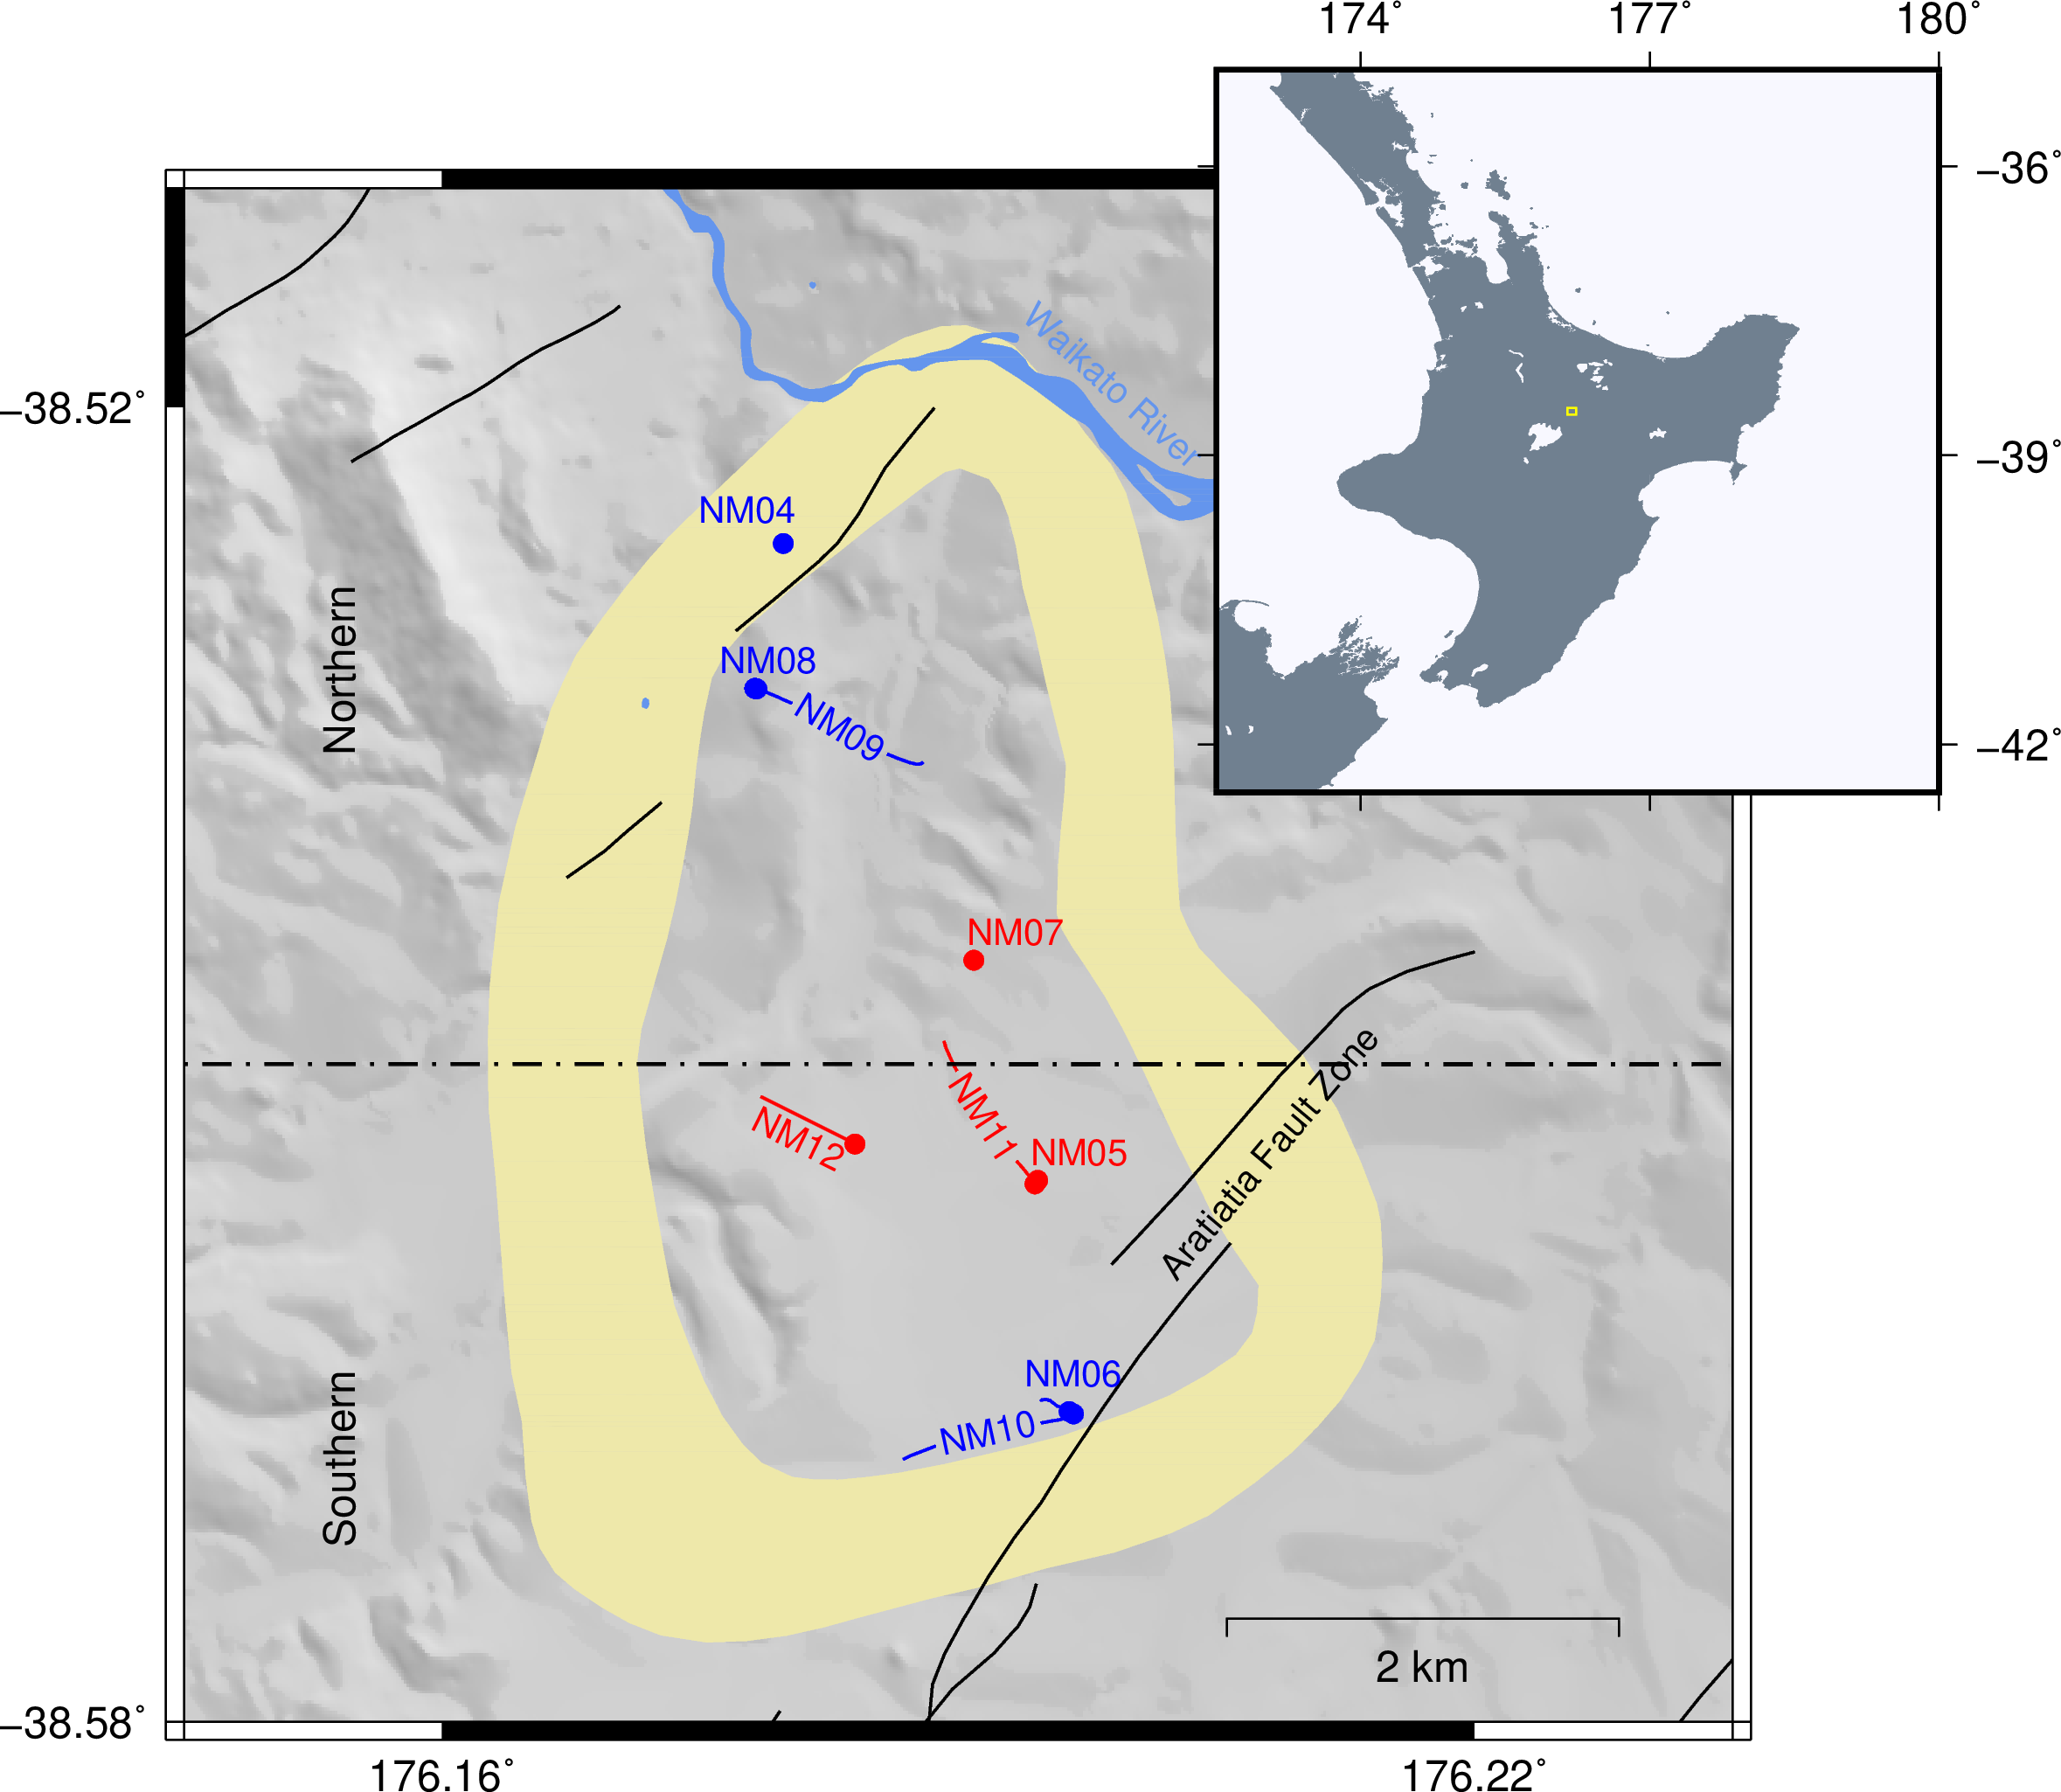
\includegraphics[width=0.70\columnwidth]{Chapter_3_Nga/figures/merc_Nga_overview_temps-wells_12-15/merc_Nga_overview_wells_12-15_original}
\caption{{Overview of the Ngatamariki geothermal field. Injection wells are shown
in blue, production wells in red with dots representing the wellhead and
lines showing the surface projection of the well tracks at depth. Wells
NM04, NM08, NM05 and NM07 are near vertical and, therefore, appear only
as dots in the figure.~ Active faults from the GNS Active Faults
Database~\protect\citep{AFDB} are shown in black. The most likely boundary
of the deep resource as published by~\protect\cite{Boseley_2010} based on
magnetotelluric surveys, is shown in yellow. The northern and southern
portions of the field, as referred to in this work, are divided at
-38.55 degrees latitude and labeled here.
{\label{795275}}%
}}
\end{center}
\end{figure}

\subsection{Mechanisms of microseismicity and permeability enhancement}
The main driver of microseismicity at Ngatamariki is the injection of cool (\textless{100}\textdegree{C}) fluid into the hot ($\sim$280\textdegree C) reservoir. It is generally accepted that fluid injection increases the pore-fluid pressure near an injection well, lowering the effective normal stress and inducing slip on suitably oriented fractures with respect to the local stress field \citep[e.g.][]{Zoback_1997,Ellsworth_2013,Langenbruch_2018}. At every point on a fracture or fault, there is a specific pore pressure increase, $\Delta{P_{crit}}$, that will lower the shear strength of the fracture\slash{fault} to the point of failure \citep{Wiprut_2000}. Injection, especially in high-temperature geothermal reservoirs, also introduces a thermal gradient in the host rock. This may produce enough stress to induce tensile failure or opening of preexisting fractures \citep{Mart_nez_Garz_n_2014}. It also reduces stress locally through thermoelastic contraction of the rock matrix, bringing the reservoir fracture network closer to or further from failure depending upon the direction of fluid flow relative to the orientation of the in situ stress state \citep{Jeanne_2014}. Furthermore, as geothermal fluid moves through a formation, it may dissolve minerals (e.g.\ calcite) out of, or precipitate minerals into, fractures. Though less well understood, this effect may play a large part in creating or destroying permeability through opening or sealing of fractures that would be likely to fail \citep{Clearwater_2015}. Injection and extraction of large quantities of fluid can also significantly change the volume of the reservoir, poroelastically influencing the distribution of stress and often leading to reservoir compaction, surface subsidence and seismicity \citep{Segall_1989,Segall_1998,Bromley_2013}. Finally, slip itself (both seismic and aseismic) transfers stress onto nearby fractures and faults, an effect that has been shown to play a role in triggering subsequent seismicity in geothermal fields and elsewhere \citep{Schoenball_2012,Catalli_2016}.

The relationship between seismicity and permeability has been widely studied in laboratory settings \citep[e.g.][and references therein]{Lee_2002}. When slip occurs on a new or preexisting fracture, asperities become offset and the permeability of that fracture increases (an effect known as self-propping), which depends on the length of the slip vector and the roughness of the fault surface \citep{Ishibashi_2018,Esaki_1999,Fang_2017}. It is commonly assumed that the permeability increase observed during injection is the result of seismic fault slip, a correlation which has been modeled for EGS cases previously (e.g.\ \citet{Baisch_2010}). It is important to note, however, that a large percentage of the permeability enhancement that accompanies well stimulation may be aseismic, as has been directly observed during a decameter-scale injection experiment described by \citet{Guglielmi_2015} and in seismic data recorded during hydraulic fracturing \citep{Das_2011}. Further evidence of aseismic slip has been inferred at the high-temperature Salton Sea geothermal field in southern California from a combined geodetic and seismic dataset \cite{Wei_2015}. \citet{Riffault_2018} have also demonstrated that, in some cases, permeability enhancement may not be coupled to detectable seismic slip at all. In the context of high-temperature geothermal reservoirs, thermal stresses induced near the wellbore may govern most of the permeability enhancement observed during well stimulation through the expansion of permeable zones \citep{grant2013thermal,siega_2014}, a process which may be aseismic.

At Ngatamariki, the dominant processes driving microseismicity have previously been interpreted to be thermal and pore-fluid pressure changes \citep{Sherburn_2015,grant2013thermal}. The Ngatamariki power plant reinjects most of the extracted fluid and, as a result, the pressure drawdown observed across the field is minor ($\sim$0.2 MPa). This suggests that reservoir compaction plays a small role in inducing local stress changes in this case \citep{quinao_2017}. However, at nearby fields that have been produced for much longer than Ngatamariki, significant pressure drawdown-related subsidence has occurred \citep{Allis_2000}. Poroelestic stress transfer resulting from rock matrix contraction and slip on fractures cannot be ruled out as possible factors affecting reservoir permeability and induced seismicity. However, in the case of the NM08 and NM10 injection tests and NM09 Stimulation A (introduced below), the injection of river water also renders unlikely the precipitation of minerals as a possible mechanism of permeability change. This cannot be said of the brine injected during the second phase of NM09 stimulation.

\subsection{Ngatamariki power plant operations} \label{Plant_ops}
Mercury Ltd., then known as Mighty River Power (MRP), began generation of electricity at Ngatamariki in October 2013 with the commissioning of an 82 MWe binary power plant. The company was granted a consent for production of 60,000 tons of geothermal fluid per day, approximately 98\% of which is currently reinjected into the deep reservoir at between 1000 and 3000 m depth. The reinjected fluid is allocated nearly evenly between the injection wells to the north (NM08, NM09) and those to the south (NM06, NM10) \citep{Clearwater_2015,buscarlet_2015}. Between June 2012 and April 2013, three of the four main injection wells were subject to some form of injection operation (Table \ref{table:operations}). Cold-water stimulation of NM08 took place between 8 June and 10 July, 2012 using $\sim$10\textdegree{}C river water. Well NM10 was drilled between late May and early August 2012, using fluid consisting almost entirely of river water, and significant fluid losses occurred after 13 July. After the completion of drilling, NM10 injection testing was conducted on 1--23 September. NM09 was drilled between September and early November 2012, with subsequent injection testing occurring in two phases. The first took place between 14 December 2012 and 4 January 2013 and the second lasted from 13 February to 6 March 2013 \citep{Clearwater_2015}, the latter using geothermal brine instead of river water. This paper focuses on the cold-water stimulation of NM08, drilling and cold-water stimulation of NM10 and cold-water stimulation of NM09.

In March 2013, as the plant was being brought online, Mercury began reinjection of brine into all injection wells including NM06, which had been drilled several years earlier. Geothermal brine at Ngatamariki is injected at a temperature of approximately 90\textdegree C. However, at times when production exceeded plant intake capacity during the early stages of plant startup, some brine bypassed the plant and was injected at temperatures of as much as 150\textdegree C \citep{Clearwater_2015}. Over the following year, injection at Ngatamariki reached a stable level of $\sim$1000 tonnes per hour (t/h) at NM09, $\sim$200 t/h at NM08 and $\sim$800 t/h at NM06. NM10 was initially an active injector but, due to the strong hydraulic connectivity between it and the production well NM05, it was phased out by mid-2015 \citep{buscarlet_2015}.\selectlanguage{english}

\begin{table}
\centering
\resizebox{\textwidth}{!}{%
\begin{tabular}{ccccccc}
    {Operation} & {Zone} & {Start} & {End} & {Injectate} & {Max Q (t/h)} & {Max Pres. (MPa)}\\ \midrule
    NM08 Stimulation  & Northern & 6-8-2012 & 7-10-2012 & River water & 175 & 2.63 (WHP)\\
    NM10 Drilling  & Southern & 5-25-2012 & 8-11-2012 & Drilling fluid & 141 & N/A  \\
    NM10 Stimulation  & Southern & 9-1-2012 & 9-23-2012 & River water & 201 & 9.3 (DHP) \\
    NM09 Stimulation A  & Northern & 12-14-2012 & 1-4-2013 & River water & 170 & 0.2 (WHP); 15.3 (DHP) \\
    NM09 Stimulation B  & Northern & 2-13-2013 & 3-6-2013 & Brine & 152 & 0.3 (WHP); 13.0 (DHP)  \\
\end{tabular}}
\caption{{Table summarizing the injection operations presented here, all of which were undertaken prior to plant startup at Ngatamariki. The maximum pressures reported in the final column are for wellhead pressure (WHP), downhole pressure (DHP) or both where present. Q denotes flow rate in tons / hour.}}
\label{table:operations}
\end{table}

\section{Data} \label{Data}
The Mercury seismic network covers an area roughly 30 km (N--S) by 15 km (E--W) with the bulk of the stations occupying an area 15 km (N--S) by 7 km (E--W) centered around the Rotokawa and Ngatamariki geothermal areas (Figure S1, supplemental materials). The majority of the instruments are either 4.5 Hz Geospace GS-11D short-period geophones or Lennartz LE-3DLite 1 Hz instruments, but the network also includes stations operated by Contact Energy (THQ2, ARAZ) at the Wairakei and Tauhara geothermal fields and nearby stations operated by the national seismic network, GeoNet (WPRZ, PRRZ, HRRZ, ALRZ) (Table T1, supplemental materials). The GeoNet stations are broadband instruments with the exception of WPRZ, which is a 1 Hz LE-3Dlite. From the beginning of 2012 until the end of 2015, the number of operational stations varied between 15 and 29. Sites NS12, NS13 and NS14 in the middle of the Ngatamariki network are 2 Hz borehole instruments installed at depths of between 200 and 514 meters below the ground surface (Figure S1, supplemental materials).

The initial earthquake catalog for this study was provided by GNS Science under contract to Mercury. The waveform data were collected roughly every three months from Mercury's data loggers and supplemented by data from nearby GeoNet stations. GeoNet data were sampled at 100 Hz while the Mercury network data were sampled at 200 Hz. For much of this study, all data were resampled at 50 Hz to reduce computational costs. Events in the initial GNS Science earthquake catalog had been automatically detected and located with the SeisComP3 software package \citep{Weber2007}. We filtered the catalog to include only these events within or immediately adjacent to the field boundaries at Ngatamariki, leaving a total of 1171 microearthquakes of local magnitudes between 0.26 and 3.17. Magnitude distance corrections were computed using events recorded by both the Mercury seismic network and GeoNet. The calibration factor for a given event-station distance, $A_0$ was calculated from $M = \log_{10}A - \log_{10}A_{0}$, where $A$ is the event amplitude at the station and $M$ the GeoNet calculated magnitude. $A_{0}$ was averaged across all stations in the Mercury network for all events recorded by GeoNet to obtain the final calibration factors. A final, static correction factor of +0.32 was applied to the Mercury magnitudes to bring them into agreement with GeoNet-calculated magnitudes (Figure S2). We relocated these events using the double-difference relocation software of \citet{Waldhauser_2000}, the results of which are shown relative to the seismic network in Figure S3 (supplementary materials). Production and injection well locations as well as flow rates and pressures at each well were provided by Mercury.

\section{Methods}
\subsection{Matched filter detection}

The small magnitudes of events, high levels of anthropogenic noise and highly-attenuating geology  at Ngatamariki make detecting microearthquakes difficult. One way to address this difficulty is to use a waveform-correlation-based detection technique. Correlation-based detection, otherwise referred to as matched-filter detection, offers improved performance over traditional, amplitude-based techniques due to its ability to detect signals in noisy data and when multiple events are closely spaced in time \citep{Gibbons_2006, Shelly_2007}. This significantly increases the number of events detected without increasing the rate of false detections and is ideal for monitoring microseismicity. Such a technique is ideally suited to areas of geothermal power generation, which are characterized by numerous noise sources and dense clusters of small seismic events.

Matched-filter earthquake detection relies on waveform cross-correlation of a
known earthquake signal or signals, referred to as templates, with continuously recorded seismic data. The following equation, which we use for this study, describes normalized cross-correlation in the time domain \citep{Chamberlain_2017}:
\begin{equation}
R(x) = \frac{\sum_{x'=0}^{x+w_{x}}(T'(x') \cdot I'(x + x'))}{\sqrt[]{\sum_{x'=0}^{x+w_{x}}(T'(x')^2 \cdot \sum_{x'=0}^{x+w_{x}}I'(x + x')^2}}
\end{equation}
Here $I'$ represents the continuous seismic data of interest and $T'$ represents the template earthquake. $x$ represents the sample in the continuous data between sample $0$ and sample $(N_{x} - w_{x})$, where $N_{x}$ is the length of the continuous data being searched and $w_{x}$ is the length of the template. $x'$ is the position within the window over which the correlation is being calculated.

Each of 1171 events taken from the GNS Science catalog outlined in Section \ref{Data} was used as a template event (Figure S3). Each template consists of one-second-long waveforms, starting 0.1 seconds before the P-phase arrival on the vertical channel at each station on which a P-pick was made (e.g. red waveforms in Figure \ref{971628}). Horizontal channels are not used due to the large uncertainties for the automatic S-picks in the GNS Science catalog. However, a length of one second ensures that both the P- and S-arrival are included in the vertical-channel template for each event due to the short travel times. A length of one second also omits most of the coda, which is incoherent for even highly similar sources. This effect is especially apparent at Ngatamariki, due to the highly-fractured reservoir, large variations in the volcanic geology (i.e.\ welded ignimbrites and ashfall deposits) and surface heterogeneity. After applying an anti-aliasing filter, waveforms were sampled at 50 Hz and filtered from 3.0 to 20.0 Hz to include the high corner frequencies of events with event-station distances of \textless5 km. Continuous seismic data were processed in an identical manner to the templates for the matched-filter routine.

To generate detections, event templates were cross-correlated with continuous
data at a rate of 50 samples per second. At each sample, the cross-correlation
coefficients for each channel of data were summed to create the network detection statistic \citep{Shelly_2007}. A detection was recorded whenever the detection statistic exceeded a threshold value, which in this case was defined as the daily median absolute deviation (MAD) of the detection statistic multiplied by eight \citep[as suggested by][]{Shelly_2007}. We refer to a template event, along with all of its associated detections, as a family.

We split all families into separate groups for northern and southern Ngatamariki
before removing duplicate detections. This allows us to account for simultaneous seismicity within both clusters, which we would expect in response to simultaneous injection at the two distinct injection zones. However, the separation of the two clusters prior to duplicate removal introduces the possibility of double-counting events detected by two templates if both templates are located in separate spatial clusters. We have checked for this case explicitly and have eliminated these cases in the final catalog presented here.

Within each spatial cluster, duplicate removal was conducted by looping through all detections in order of descending detection statistic and removing detections within a user-defined time buffer of two seconds. We adopted two seconds for the time buffer after a visual review of template events revealed
numerous cases of near-repeating seismicity with inter-event times of 3--5 s.

Visual inspection of a subset of the detection waveforms showed that false detections occurred at a rate of approximately 1--3 false detections per day. However, the quantity of detections makes visual review of the entire detection catalog impracticable. Therefore, we employ a sequence of thresholds based on the cross-correlation between the template and detected waveforms to exclude lower-quality events. We do this during both the location and magnitude calculations detailed below. Applying these correlation cutoffs has the effect of suppressing false detections in the final catalog that we use in this analysis. As a final quality assurance step, we visually inspected hundreds of waveforms from the final catalog in order to manually pick first motion polarities and did not encounter a false detection.

\subsection{Detection location} \label{methods_location}
After removing duplicate detections, P-picks for each of the newly detected
events were made at each channel included in the template. For each station, template waveforms were correlated with the detected waveform over a 0.2 second window centered on the detection time. Picks were recorded at the time corresponding to the highest correlation value within that window. However, if the correlation value of the template and detected waveform fell below 0.4, the pick was discarded. We retained all events with more than five picks and discarded those with five or fewer. For the retained events, we then made automatic S-picks \citep{mroczek2016shear} using the method developed by \citet{Diehl_2009} and modified by \citet{Castellazzi_2015}. These events were then located with the nonlinear location program \href{http://alomax.free.fr/nlloc/}{NonLinLoc} \citep{Lomax_2014} using a preliminary 1-D model computed in VELEST \citep{Kissling_1994,sewell2017}(table S1). As a final step, the entire catalog was relocated using the double-difference relocation program GrowClust \citep{Trugman_2017} with differential pick times generated using the Python package hypoDDpy \citep{lion_krischer_2015_18907}. The final double-difference relocations are shown in Figure \ref{827409}.

\subsection{Magnitudes} \label{methods_magnitudes}
To compute the magnitude of the events detected by the matched filter,
we used the method described by \citet{Shelly_2016}. This technique uses pair-wise relative amplitudes between a template event and each of its detections to compute relative moments. This approach computes the relative amplitude, $\alpha$, as
\begin{equation}
\alpha = \frac{v[2]}{v[1]}
\end{equation}
where $v[2]$ and $v[1]$ are the second and first elements, respectively, of the first row of the 2$\times$2 matrix $V'$ in
\begin{equation}
M = U\Sigma V'
\end{equation}
where $M$ is the singular value decomposition of a data matrix containing both the template and the detected waveform on a single channel. The rows of $V'$ are the right singular vectors which map the weight of the left singular vectors, $U$, to the original data vectors. Because the template and detected waveforms in the data matrix are inherently similar, the first left singular vector, $U_0$, should describe only a difference in amplitude between template and detection. The relative amplitude between the two events can therefore be estimated as the ratio of the second and first elements, $v[2]$ and $v[1]$, of the first row of $V'$.

We calculated relative amplitudes only when the cross-correlation coefficient between the template and detection exceeded 0.6 at any given station. Again, we note that template events only contain waveforms for the vertical channels. For those events recorded by a minimum of four stations exceeding the correlation threshold, we calculated the relative moment as the median of the relative amplitudes, following \citet{Shelly_2016}. We note that, because the relative amplitudes are calculated from two waveforms recorded at the same station, there is no need to remove the instrument response.

This approach has proven to be more robust in the presence of relatively dissimilar waveforms than the method of \citet{Rubinstein_2010}, which assumes high correlation coefficients between all events in a family (e.g.\ $\geq$0.85). In the Ngatamariki case, scattering and attenuation effects produce waveforms exhibiting lower degrees of similarity than typical repeating or near-repeating seismicity (e.g.\ along the San Andreas \citep{Rubinstein_2010}).

We used the GNS Science $M_{L}$ (as described in Section \ref{Data}) to calibrate the relative moment calculations from the method above and produce $M_{L}$ estimates for matched-filter detections. This was done by first converting the template local magnitudes to moment magnitudes using the scaling relationship
\begin{equation}\label{ristau}
M_{L} = 0.88M_{w} + 0.73
\end{equation}
determined for locally detected, shallow New Zealand earthquakes \citep{Ristau_2009} and then converting to seismic moment using the equation:
\begin{equation}
M_w = 2/3\log_{10}M_{0} - 9
\end{equation}
\citep{Hanks_1979}. Knowing the relative moment of the template event from the procedure outlined above, we then determined the relationship between the relative moments and actual moment which allowed us to convert relative moments to $M_w$ and then back to $M_L$ using Equation \ref{ristau}.

\subsection{Focal mechanisms and stress inversion}
Focal solutions for selected events were calculated from P-arrival polarities using the Bayesian focal mechanism determination program of \citet{Walsh_2009}. Here, we present only focal mechanism solutions for the 86 events that occurred prior to plant startup in March 2013 and that had sufficiently high signal-to-noise ratio for the arrival polarities to be manually picked. These focal mechanisms were then used to invert for the stress parameters and the direction of maximum horizontal compressive stress (S$_{HMAX}$) within the northern and southern clusters separately, using the methodologies of \citet{Arnold_2007} and \citet{Lund_2007}.

\section{Results}
\subsection{Matched-filter detection}\label{MF-results}
Starting with the 1171 template events in the automatically detected catalog provided by GNS Science, we added 76,286 detections after matched filtering, creating a total catalog of 77,457 detections. At Ngatamariki, seismicity in both the GNS Science catalog and the matched-filter catalog falls into two spatial groups, which we refer to hereafter as the northern and southern clusters. We delineate the templates broadly by latitude whereby the northern cluster contains all templates located north of -38.55 degrees and the southern cluster contains all templates to the south (Figure \ref{795275}). The northern cluster consists of 432 template events, which generated 25,482 detections. The southern cluster consists of 739 template events, which generated 50,804 detections. Two representative detections for a single template from the northern cluster are shown in Figure \ref{971628}.\selectlanguage{english}

\begin{figure}[h!]
\begin{center}
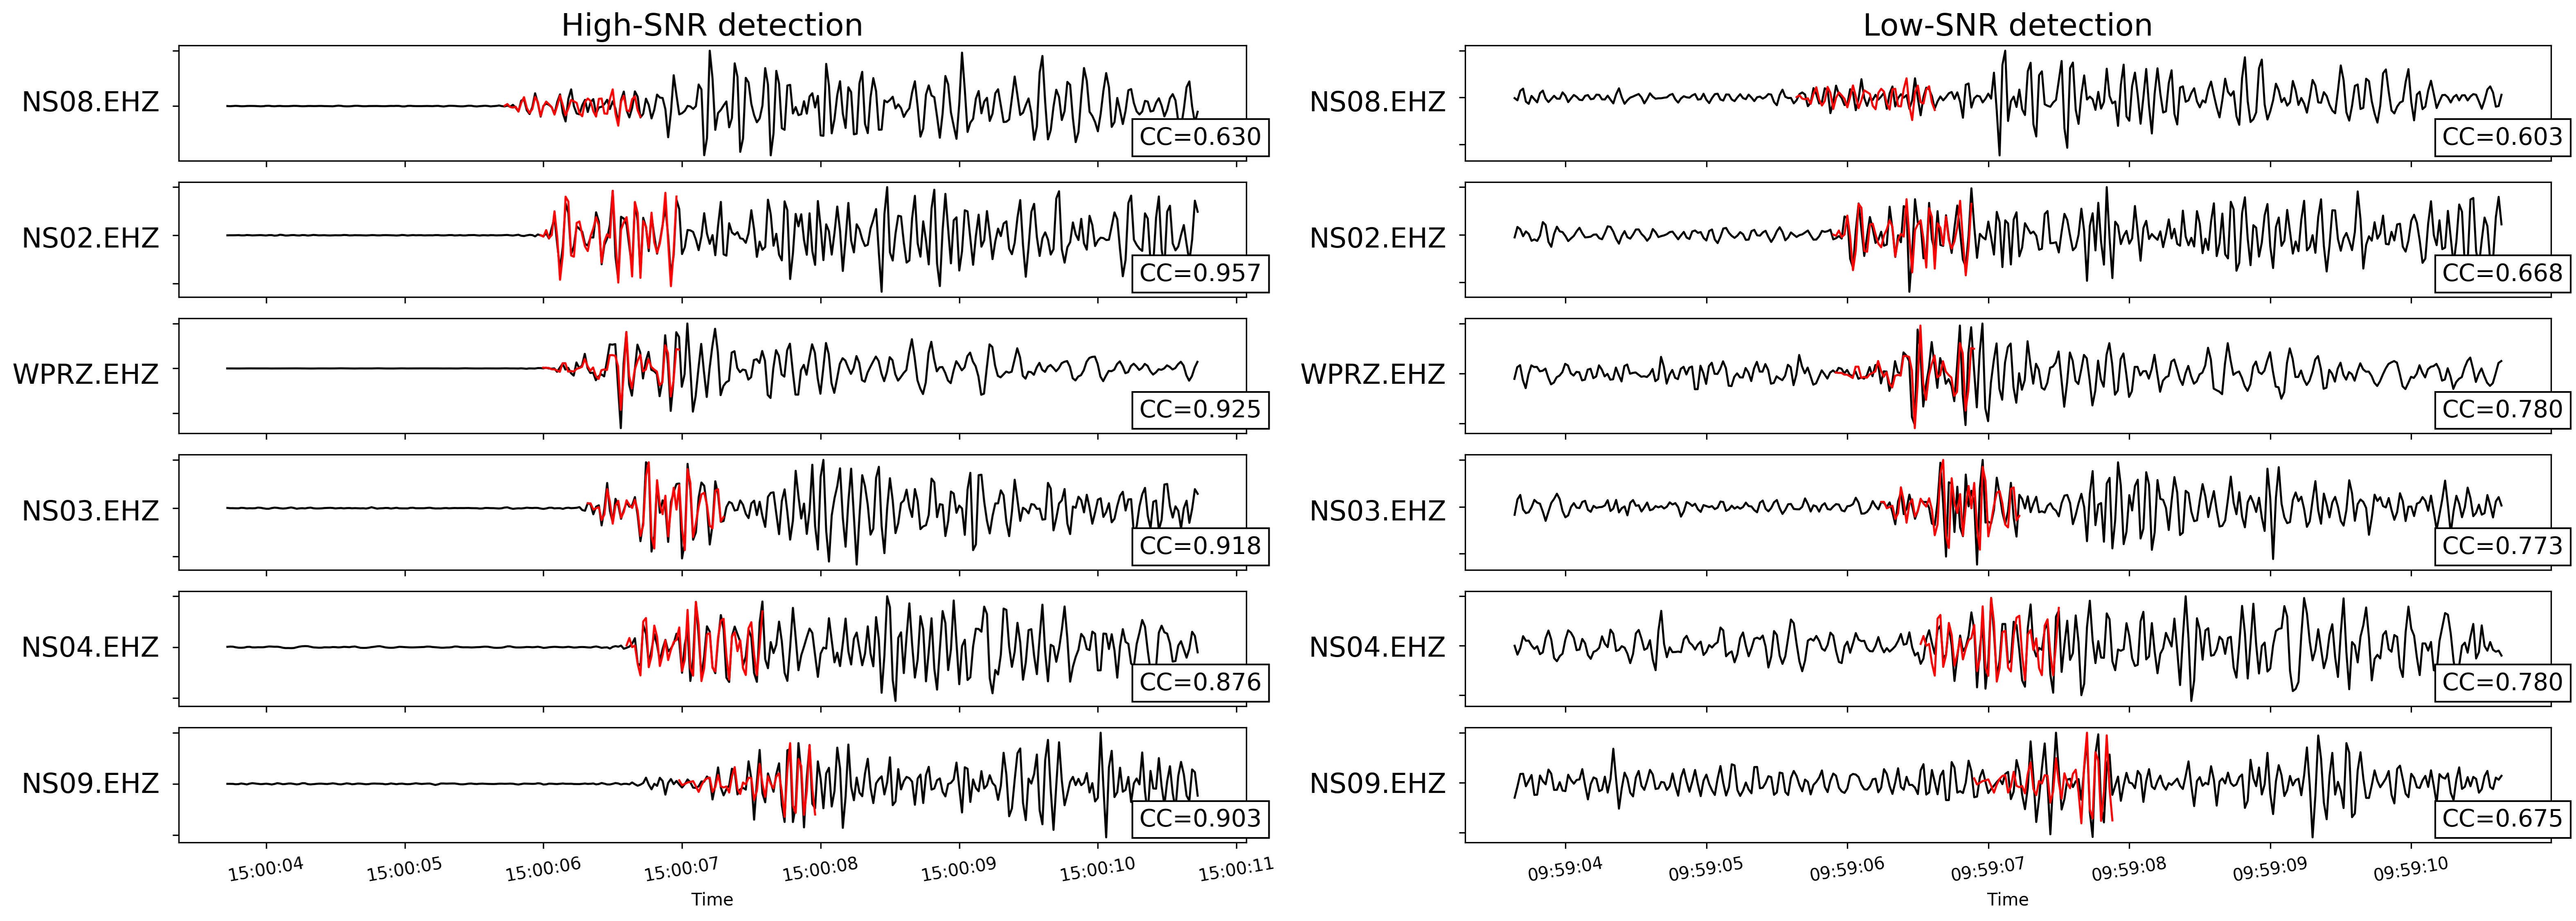
\includegraphics[width=1.00\columnwidth]{Chapter_3_Nga/figures/2012sora453983_20120619_051750460000/det_example_publication_original}
\caption{{Example detections of two events by template 2012sora469246
(signal-to-noise ratio of $\sim$50 and $\sim$3
respectively). The 1 s templates (in red) are overlain on 10 s of
continuous data around the time of detection (black). The
M\textsubscript{L} 0.62 template event occurred on 22 June 2012 and
detected mostly events that occurred during the stimulation of well NM08
between 6 June and early July. The detection on the left represents a
detection of a separate, yet highly-similar, template event (template
2012sora469256) which occurred approximately ten minutes after the
template event shown here. The detection on the right is a
newly-detected event.
{\label{971628}}%
}}
\end{center}
\end{figure}

\subsection{Event location} \label{location_results}
We calculated preliminary locations for 41,114 events of the 77,457 total detections. Of the 5981 of these events for which we calculated magnitudes, we were able to relocate 2554. Given that events detected by the matched-filter method are, by design, similar to the template event that detected them, the locations of the detections should closely match the locations of the template events. Figures \ref{827409} and S3 show the detected and template events, respectively, plotted with depth and colored by their date of occurrence (blue for earlier in the dataset, pink for later).

In northern Ngatamariki, most events occur within a cloud of seismicity extending from $\sim$1500 to 2500 meters below sea level (m bsl). This cloud is spatially coincident with the dominant feedzones in well NM09 at between $\sim$1600--1800 m bsl (Figure \ref{827409}). The injection rate during normal power plant operation is roughly 1100 t/h into NM09 and $\sim$300 t/h into NM08. During the stimulation of NM08, seismicity occurred within a narrow, NW-dipping band at $\sim$2200 m bsl. These events likely define the extent of a suitably-oriented fault that was activated during the treatment and which is discussed in more detail in Section \ref{NM08_stimulation}.

In the south of the field, seismicity occurred in a cluster at depths of $\sim$2000--3000 m bsl, elongated in the NE-SW direction, and sub-parallel to the strike of the Aratiatia Fault Zone (Figure \ref{795275}). These depths coincide with the depths of the major feedzones in injection well NM06, not with the feedzones in NM10. Over the entire four-year dataset, seismicity in the southern injection zone migrates from SW to NE. We attribute this migration to a shift in injection strategy in this part of the field. Originally, injection was split equally between NM10 and NM06, but by 2015 all injection in the south was into NM06 due to rapid returns from NM10 to production well NM05 \citep{buscarlet_2015}.

The depth of seismicity in southern Ngatamariki is greater, on average, than in the north. In the south, hypocentral depths correspond to the depth of the Rotokawa Andesite and the lower Tahorakuri Formation \citep{Chambefort_2014} with shallower seismicity nearer to the production wells than the injection wells. In the north, below $\sim$2000 m bsl, the reservoir is dominated by the intrusive body \citep{Chambefort_2014}. The seismicity depth cutoff near both injection zones is likely related to the depth of permeable zones in the wells \citep{massiot_2012,nm09_report,nm10_report}. In the north, relatively little seismicity occurs within the bounds of the impermeable intrusive body and in the south most events are confined to the Rotokawa Andesite, which is known to be heavily fractured \citep{nm10_report}. The high temperature within the field likely also plays a role in controlling where microearthquakes are able to nucleate. Bottomhole temperatures for the northern injection wells reach $\sim$280\textdegree C and production well NM07 reaches almost 290\textdegree C, approaching the brittle-ductile transition for quartz-bearing rock \citep{Scholz_1988}. In contrast, the maximum temperatures in the southern injection zone reach only $\sim$260\textdegree C and are located away from the main upflow in the field (between NM07 and NM08/09) \citep{Chambefort_2016}. This temperature differential likely governs the difference in the depths of seismicity between the two injection zones, as the host rock should deform brittly to greater depths in the south than in the north.\selectlanguage{english}

\begin{figure}[h!]
\begin{center}
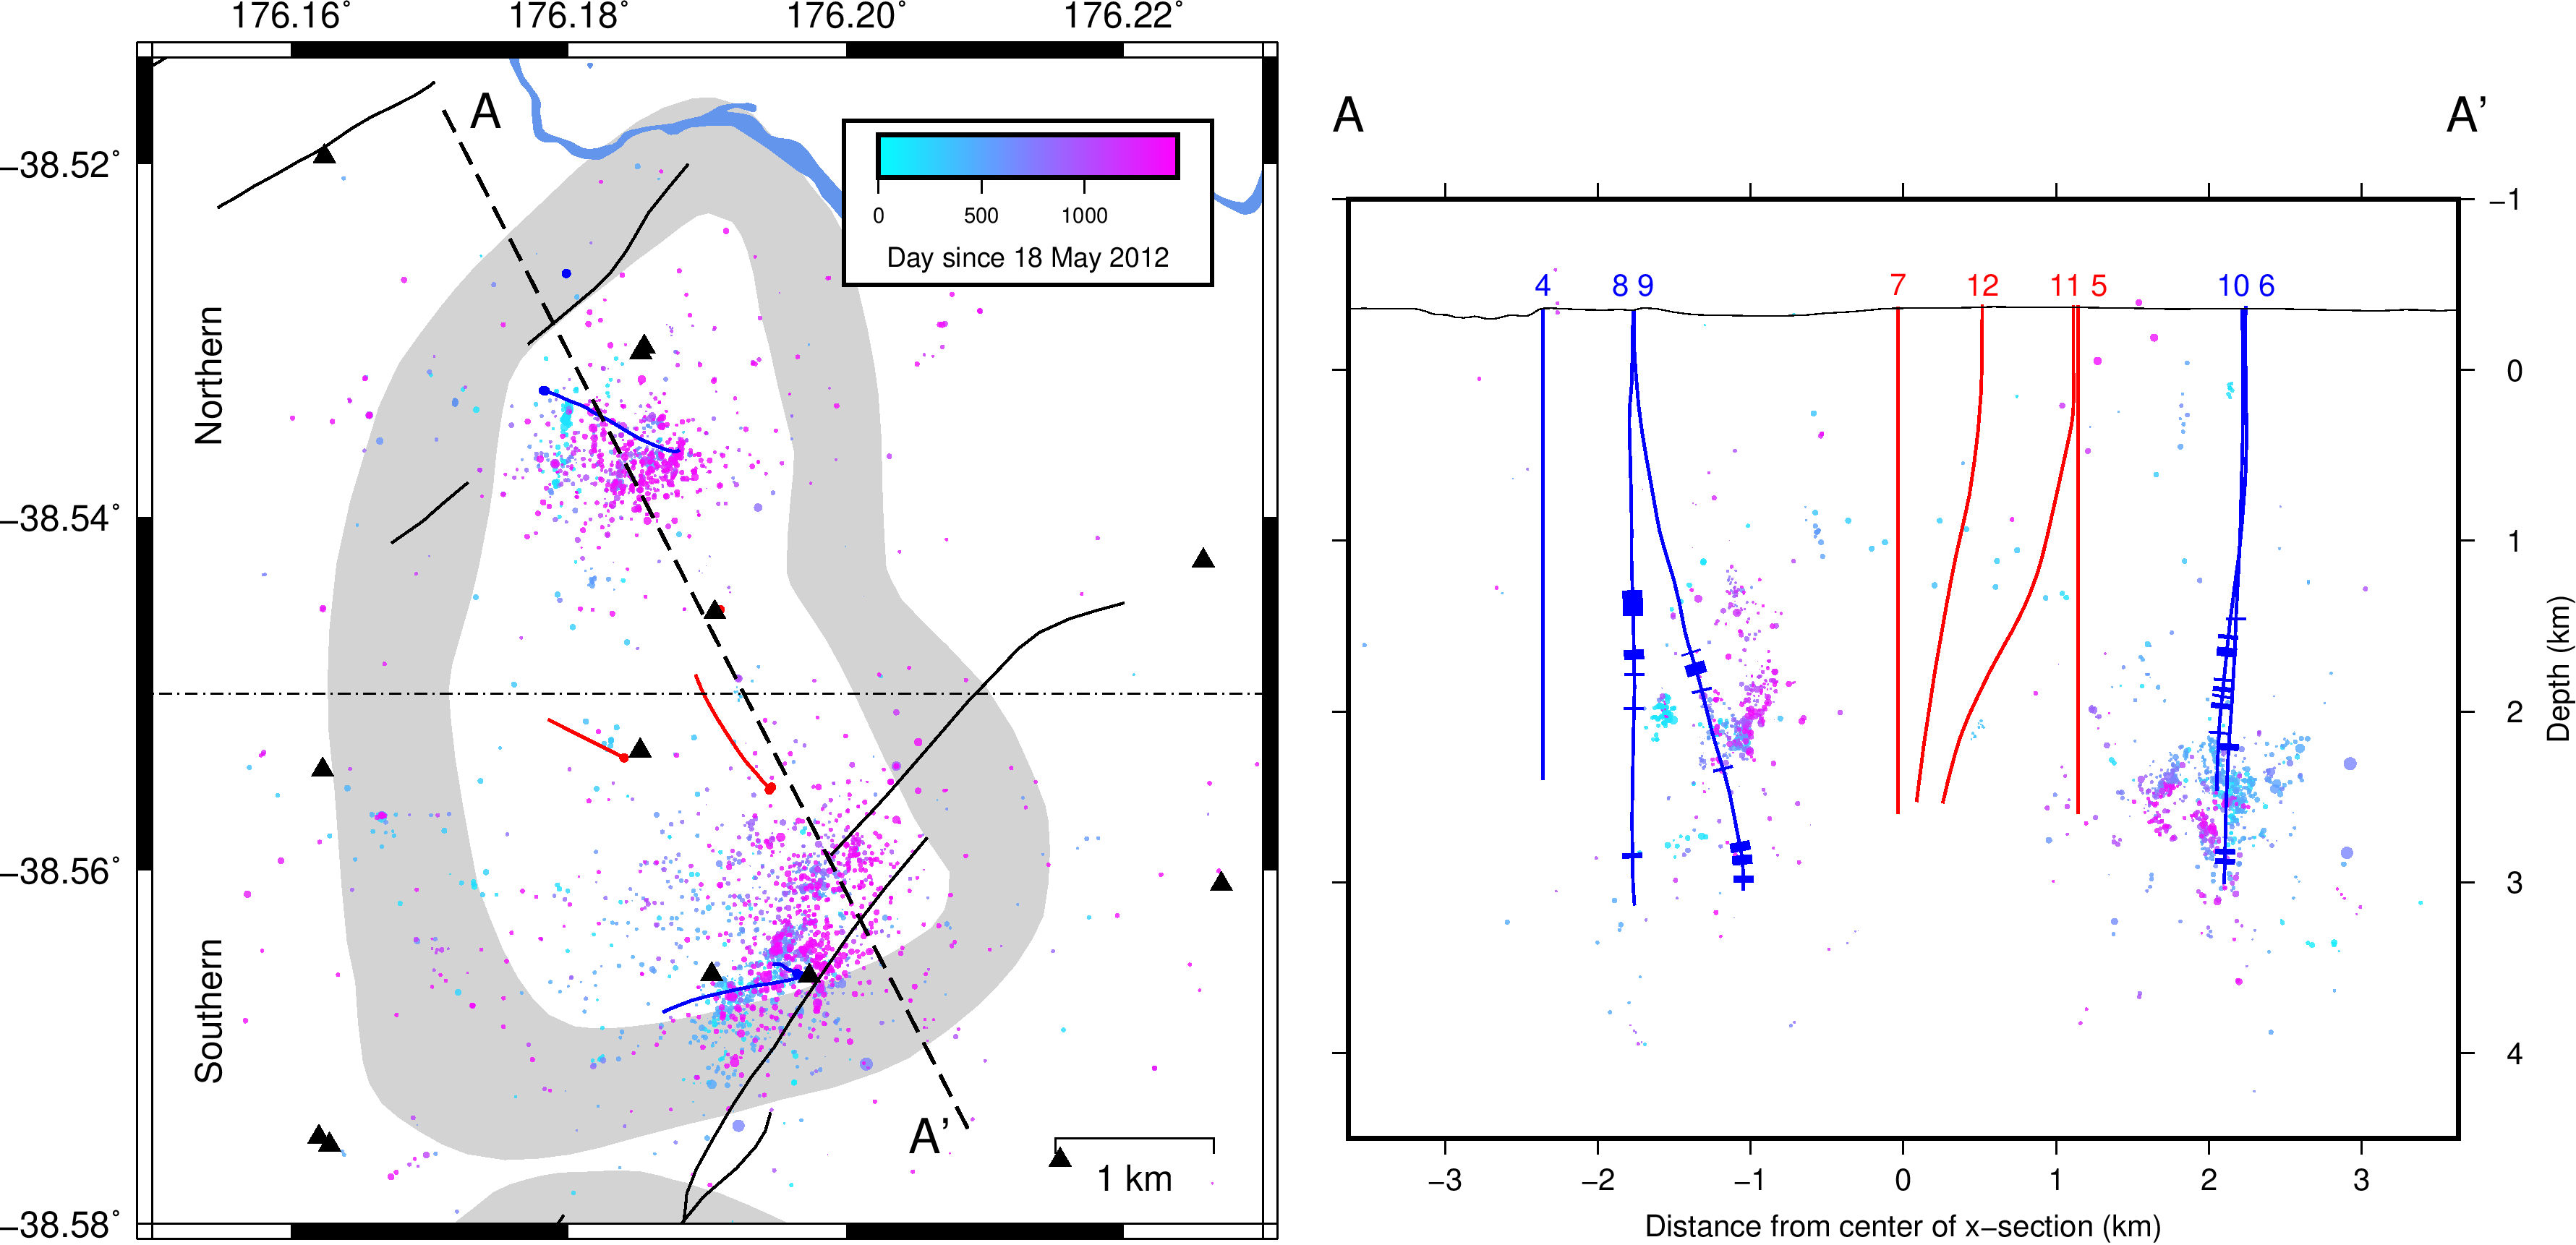
\includegraphics[width=1.00\columnwidth]{Chapter_3_Nga/figures/mrp_hypoDD_Nga_detections_hypoDD/mrp_DD_Nga_dets_GC_11-28-18_original}
\caption{{Relocated Ngatamariki seismic catalog for May 2012 through November of
2015 using the double-difference relocation method
of~\protect\citet{Trugman_2017}. Production (red) and injection (blue) wells are
shown with circles representing the wellhead and lines representing the
surface projection of the wellbore at depth. In cross-section, the major
feedzones in each injection well are shown as wide, blue rectangles.
Events are colored by the date on which they occurred and scaled by
their magnitude (M\textsubscript{max~}= 3.1). Teal corresponds to the
start of the dataset and pink to the end. Black triangles denote
locations of seismic stations. The northern and southern portions of the
field are divided by a dash-dotted line and labelled.
{\label{827409}}%
}}
\end{center}
\end{figure}

\subsection{Magnitude}
We calculated magnitudes for 3725 of the 41,114 located events using the methodology outlined in Section \ref{methods_magnitudes}. This large drop in the number of events is a result of the stringent correlation cut-off imposed ($\geq$0.6 at four or more stations, see Section \ref{methods_magnitudes}), which ensures we retain only high-quality events. Figure \ref{121528} shows the frequency-magnitude distributions for both the GNS Science catalog (dotted lines), constituting the original template events, and the detected events for which we could calculate a local magnitude (solid lines). Here we show the catalog separated into northern and southern clusters. In both clusters, the additional matched-filter detections decrease the minimum magnitude in the catalog to less than zero.

We determine the b-values for the matched-filter catalogs for a magnitude of completeness ($M_c$) calculated using the `maximum curvature' method \citep{Wiemer_1997}. However, we note that, due to the gradual roll-off of these distributions at lower magnitudes (especially for northern Ngatamariki), the `maximum-curvature' estimation method likely underestimates M$_C$ \citep{Wiemer_2000}. Notably, the inclusion of the matched-filter detections does not appreciably lower the magnitude of completeness of the catalogs here, in contrast to what has been shown elsewhere (e.g. \citet{Shelly_2016}). Regardless, the original catalogs were not complete even at higher magnitudes, as suggested by the higher numbers of matched-filter detections for events above $M_L$ 2.0 when compared to the GNS Science catalog.

We suggest that the difference in b-value between the northern and southern clusters (1.84 and 1.20 respectively) reflects a difference in the sizes of fractures and faults that are hydraulically connected to nearby injection wells. The entire field is extensively fractured, as indicated by the available image logs of the injection wells \citep{nm09_report,nm10_report,massiot_2012}, but in the south the active Aratiatia Fault Zone intersects injection wells NM06 and NM10 \citep{nm10_report}. The structures associated with this fault zone may be larger than those in the less-permeable northern portion of the reservoir where active structures are harder to identify \citep{massiot_2012}, allowing for larger-magnitude events to nucleate. During injection operations elsewhere, higher b-values ($\sim$1.5-2.0) have been observed nearer the injection point where high pore fluid pressures can induce slip on fractures subject to low differential stress \citep[e.g.][]{Bachmann_2012}. Slip on these less-stressed fractures may be the explanation for higher b-values at injection sites and volcanic regions \citep{Wiemer_1998}. This may also affect the b-values at Ngatamariki, where WHP in the northern injection zone is consistently $\sim$0.5 MPa higher than in the south.\selectlanguage{english}

\begin{figure}[h!]
\begin{center}
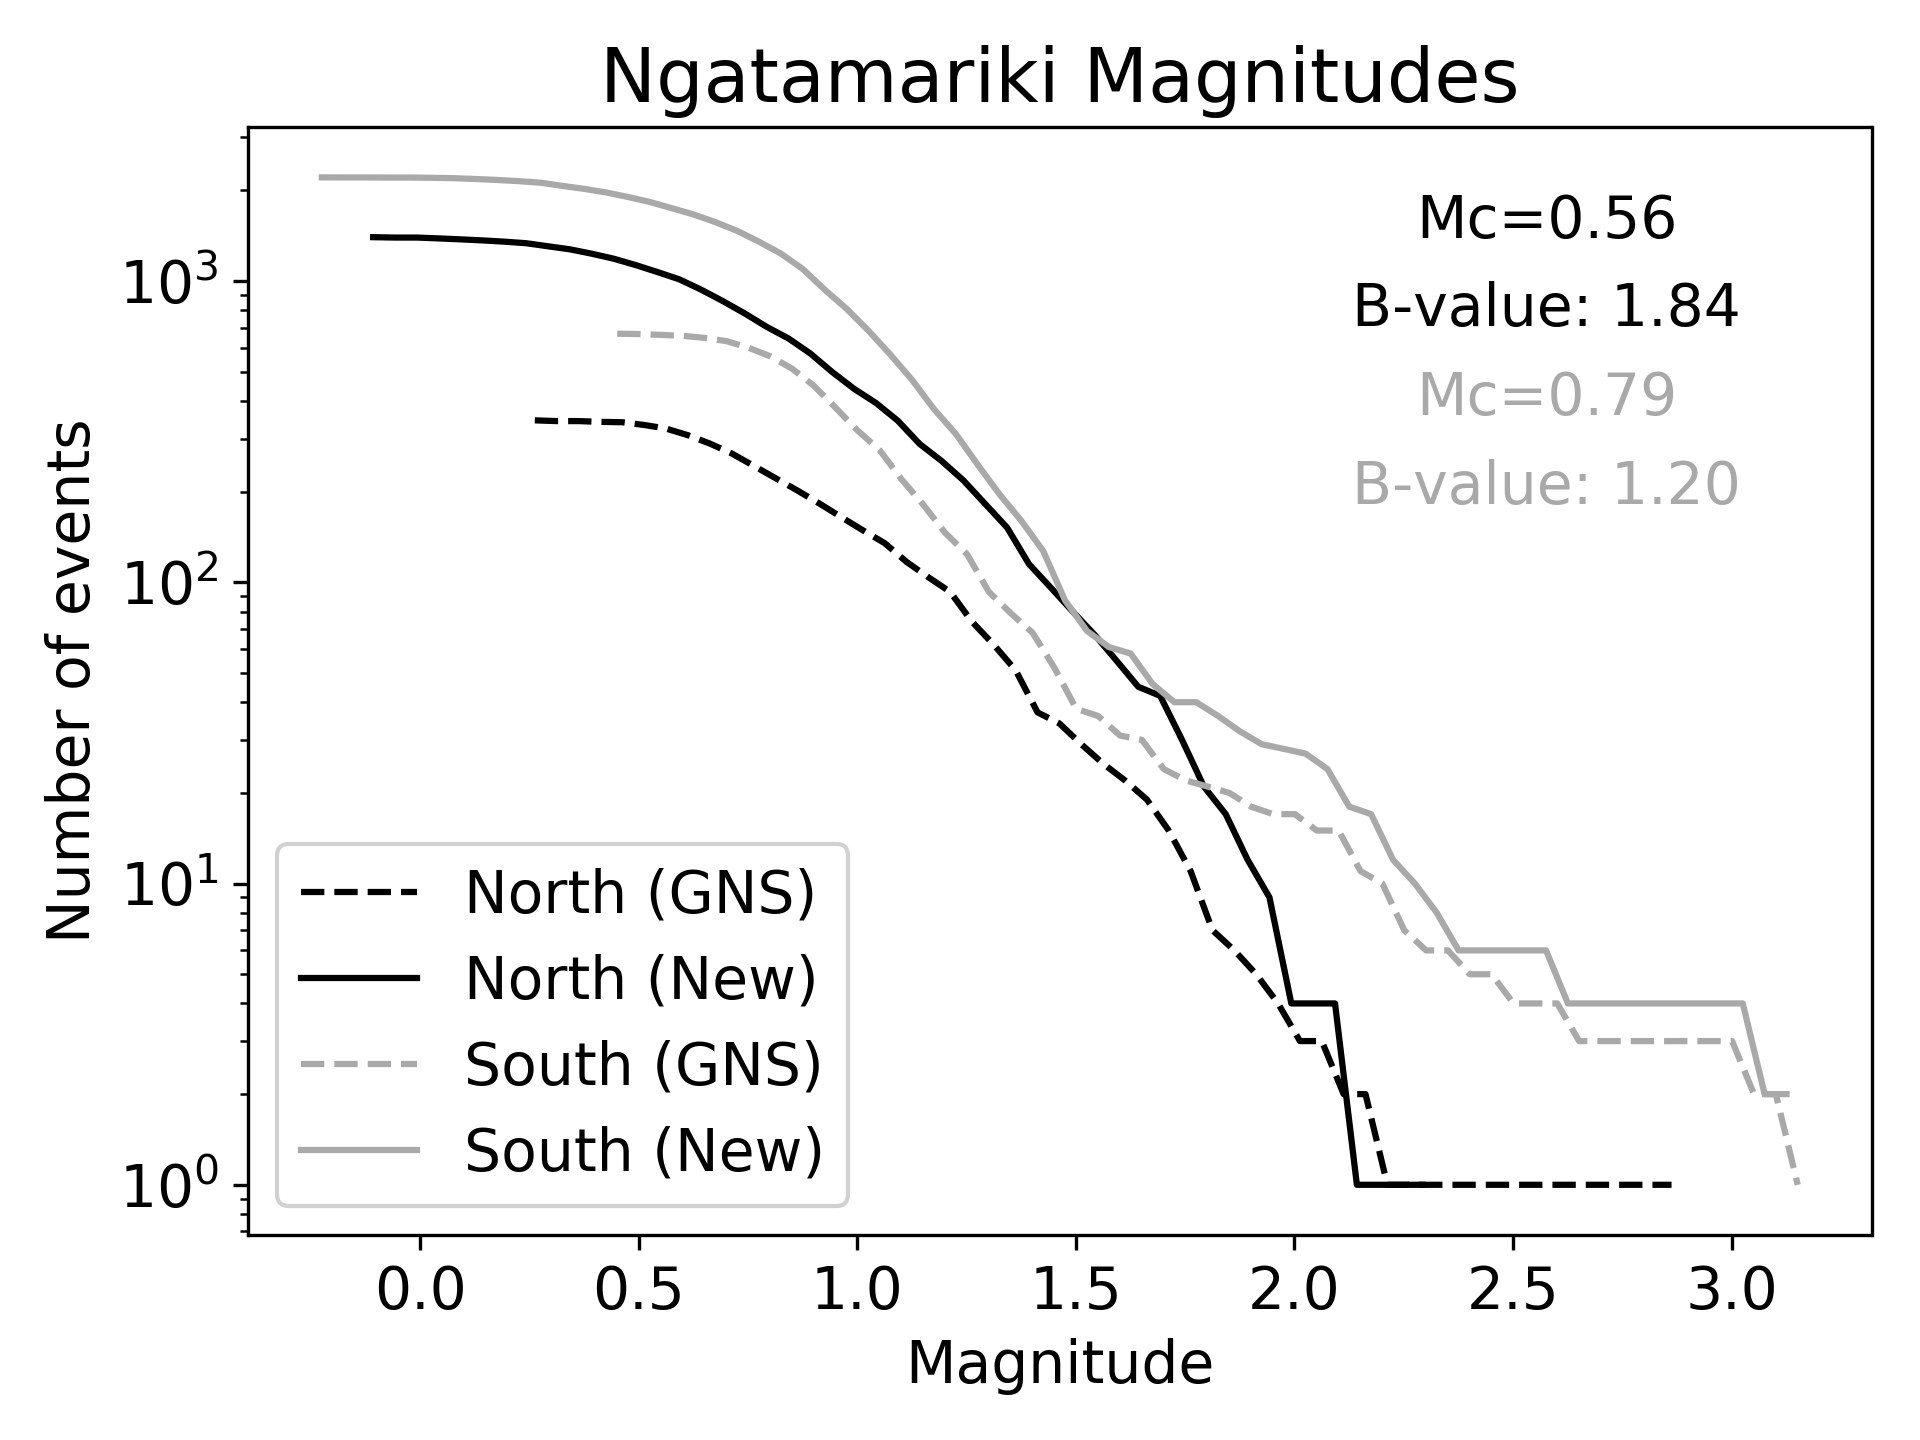
\includegraphics[width=0.70\columnwidth]{Chapter_3_Nga/figures/NgaN_min4_SVD1-5_PCA_mags_vs_temps/Nga_cumulative_bval_plots_combined_12-5_original}
\caption{{Cumulative frequency-magnitude distributions of the GNS Science catalog
of templates (dotted lines) and the final matched-filter catalog (solid
lines) for 2012-2015. Northern and southern Ngatamariki (Nga N, Nga S)
are shown in black and gray, respectively. The magnitude of completeness
is calculated using the maximum curvature method \protect\citep{Wiemer_1997} .
Calculated values of M\textsubscript{C~}and b are noted in the top
right.
{\label{121528}}%
}}
\end{center}
\end{figure}

\section{Discussion}\label{discussion}
Injection wells NM08, NM09 and NM10 underwent injection testing before the commissioning of the Ngatamariki power plant in 2013. These tests provide us the opportunity to study the seismic response to a number of isolated injections without contamination from concurrent injection from nearby wells. Below, we discuss each of these tests in detail and relate the characteristics of the accompanying seismicity to the injection parameters and geology in the respective part of the reservoir. Where possible, we calculate the well injectivity index which we use as a proxy for near-well reservoir permeability \citep{Watson_2013}. Typically, injectivity varies as $t^{n}$ where $t$ is time since the start of injection and $n$ takes a value between 0.1 and 1.0 for most geothermal wells \citep{Clearwater_2015,grant2013thermal}.

\subsection{Northern Injection Zone}
\subsubsection{NM08 stimulation}\label{NM08_stimulation}
Starting on 8 June 2012, NM08 underwent a cold-water stimulation treatment, accepting $\sim$66,000 m$^3$ of water over a period of approximately one month. This was the first injection test in the field and it triggered a sharp increase in the rate of microseismicity, which occurred predominantly in one cluster at the depth of the well's main permeable zone at $\sim$2000 m bsl (Figure \ref{645772}). This sub-planar cluster strikes $\sim$192\textdegree and dips $\sim$66\textdegree, centered on a depth of roughly 2000 m bsl. This is consistent with measurements of fracture orientation made from image logs, which suggest a dominant NE--SW strike for fractures intersecting the well and a dominant NW dip over this depth interval \citep{massiot_2012}. Flow rate, wellhead pressure and injectivity index are shown in Figure \ref{645772}.

Figure \ref{645772} shows the cumulative number of microseismic events during the NM08 stimulation, which included two phases of injection. The first, starting on 8 June, 2012 did not immediately trigger an increase in the rate of seismicity. Instead, there was a period of approximately ten days during which there were no detected events. We interpret this period to correspond to near-field pressurization of the reservoir (NF) followed by pressure breakthrough (BT) to a highly-permeable fracture zone (Figures \ref{645772} and \ref{740510}). This period of testing involved a step-rate injection test in which the WHP response was observed for incremental changes in flow rate. Following this period, on 15 June (middle of BT, Figure \ref{645772}) the injection was changed from a steady-flow to a steady-pressure regime in which flow rate was allowed to vary. This change also corresponded to a modest increase in both the injection rate and WHP. Roughly two days after this change, the rate of seismicity increased to between 5 and 12 events/day in the area of NM08 and this increased rate was maintained until the first phase of injection ended on 26 June (FZ1, Figure \ref{645772}), accompanied by an abrupt halt to seismicity.

Phase two of the stimulation began on 1 July, 2012 (start of RP, Figure \ref{645772}) at slightly higher flow rates than previously ($\sim$150 t/h). Again, the rate of seismicity did not immediately increase once the second phase of injection began. There was a delay of approximately four days before the flow rate was increased to $\sim$175 t/h with an accompanying increase in WHP of approximately 0.5 MPa (FZ2 Figure \ref{645772}). Following this increase, the rate of seismicity increased to 23 events per day (T5), slightly higher than the levels encountered during phase one. This activity ceased as soon as injection was halted on 9 July, bringing the total number of events during the stimulation to 122. The maximum $M_{L}$ during the entire stimulation was 2.1.\selectlanguage{english}

\begin{figure}[p]
\begin{center}
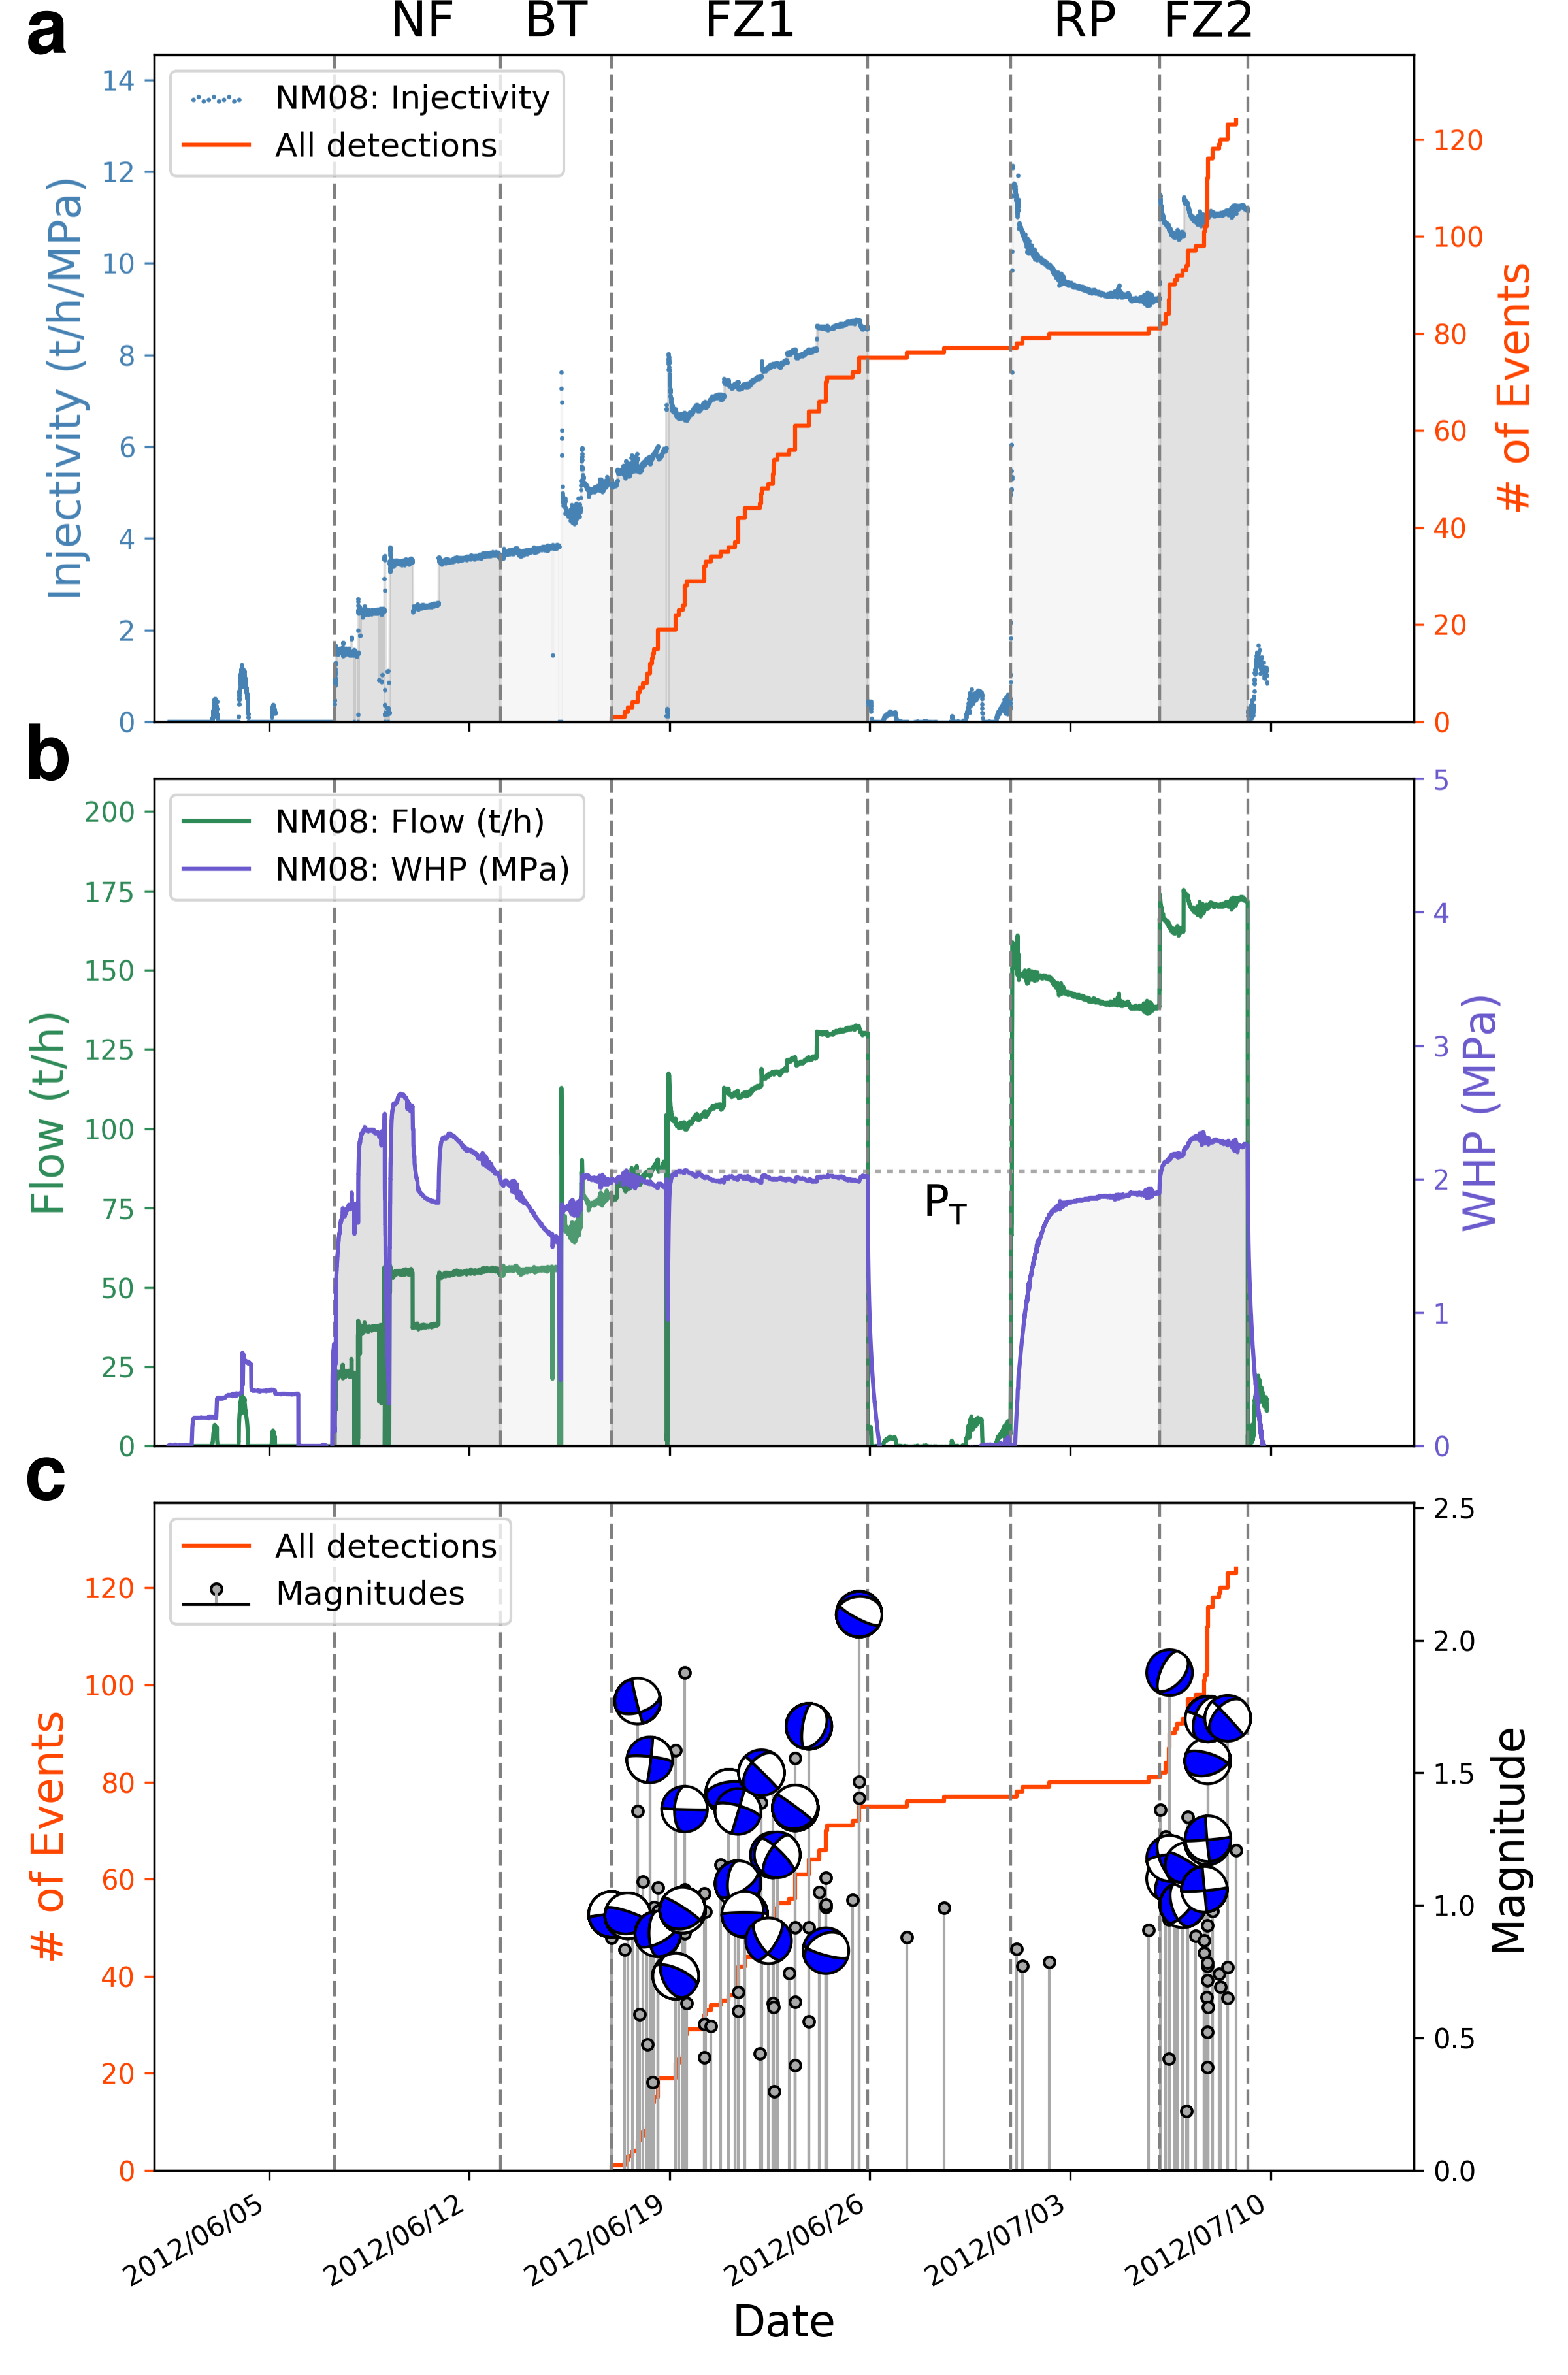
\includegraphics[width=0.84\columnwidth]{Chapter_3_Nga/figures/Multiplet_95_vs_flow_rate/Full_final_cat_flow_WHP_mags_FMs_diffusion_NM08_Stim_II_11-7_GrowClust_no_diffs_lines_gray_labels_12-5_original}
\caption{{Summary of seismicity and injection parameters during the cold-water
stimulation of NM08. A) Cumulative seismicity vs. injectivity index, B)
wellhead pressure vs. flow rate and C)~Local magnitudes and available
focal mechanisms solutions for the stimulation of NM08. Labels at the
top of the plot delineate the following periods of interest: NF:
near-field pressurization of the fracture zones surrounding the dike
swarm, BT: breakthrough of pressurization from the near-well reservoir
to the seismically-active fracture zone, FZ1 and FZ2: fracture zone
pressurization and associated seismicity, RP: renewed pressurization of
the near-well reservoir. Once the fracture zone pore-fluid pressure
exceeds the maximum induced pressure during FZ1 (P\textsubscript{T}),
seismicity is again induced. These periods are detailed in the schematic
in Figure~{\ref{740510}}.
{\label{645772}}%
}}
\end{center}
\end{figure}

Assuming that NM08 is hydraulically connected to a set of fractures, we expect seismicity to occur once an induced pressure-front has reached a critically-stressed subset of fractures in the local stress regime. The advance of the induced pressure front is controlled by the hydraulic diffusivity of the reservoir, which is closely linked to the reservoir permeability. This relationship has led other groups to develop Seismicity-Based Reservoir Characterization (SBRC) to infer diffusivity from the location and occurrence time of induced seismicity \citep[e.g.][]{Shapiro_2002,Shapiro_2009,Parotidis_2004,Jeanne_2015deformation}. At Ngatamariki, and at most other naturally-fractured reservoirs, flow is controlled not by matrix permeability but by the spacing and permeability of fractures \citep{Grant_2011}. If we consider a large enough volume of the reservoir, relative to the fracture spacing, SBRC can be useful in estimating a bulk reservoir diffusivity from the occurrence of seismic events. However, if flow is concentrated in a small number of highly permeable fracture zones (highly anisotropic permeability), as is the case at Ngatamariki, SBRC performs less well in describing reservoir properties. Nevertheless, we have fit a number of curves to the seismicity catalog for each of the injection scenarios detailed in this work (supplemental materials).

The timing and location of seismicity during the stimulation of NM08 provoke a number of questions:
\begin{enumerate}
    \item Why does seismicity lag behind the starts of injection by up to ten days?
    \item Conversely, why does seismicity stop immediately following a halt of injection?
    \item Why are the increase in injectivity index and seismicity poorly correlated in time?
\end{enumerate}

Seismicity trails injection by ten days at the outset of the stimulation, and again by four days at the start of phase two (NF and RP, Figure \ref{645772}). In the first tens of minutes following the start of injection, drilling-related degradation of near-well permeability (i.e. positive skin effects \citep{Grant_2011}) may have contributed to a delayed pressure response between the well and reservoir. However, as the seismic lag time was of the order of days, positive skin effects (normally on the order of hours) cannot account for this observation \citep{horne1995modern}. We propose that the lag is due to geologic heterogeneity in the Tahorakuri volcaniclastic succession that hosts the reservoir, which defines where the permeable zones of the well are located, as well as the orientation of the fracture network.

The main permeable zone of NM08, which coincides with the depth of seismicity during stimulation, is defined by a series of mafic dikes or sills \citep{Chambefort_2014,massiot_2012} (Figure \ref{740510}). Image log quality at this depth is poor, and the orientations of these dikes is poorly constrained \citep{massiot_2012}, but their emplacement orientation is likely to have been controlled by the prevailing stress field 0.64--0.79 Ma \citep{Chambefort_2014} and related to the emplacement of the tonalite intrusive at the bottom of the well (Figure \ref{740510}). If we assume that flow is concentrated within the damage zone surrounding the dikes and/or within the dikes' internal structures (such as cooling joints or flow bands \citep{Massiot_2017}), it may be that these structures are not optimally oriented for failure in the current stress regime. Although the prevailing tectonic environment during emplacement of the intrusive was similar to that of the present (i.e.\ active rifting \citep{Wilson_2016}), highly active volcanism in the TVZ, including the subsequent formation of the adjacent Whakamaru caldera (0.35 Ma), would likely have modified the Ngatamariki stress state \citep{Wilson_1995}.

We hypothesize that initial flow from NM08 was concentrated in these non-critically-stressed dike-related structures, and therefore did not trigger detectable seismicity (NF Figures \ref{645772}, \ref{740510}). In this case, the time lag in seismicity corresponds to a period of near-field pressurization during which NM08 was not hydraulically connected to the fracture zone defined by the hypocenters in Figure \ref{532034} (striking 192\textdegree, dipping 66\textdegree NW). If we consider an alternative scenario, in which NM08 was always hydraulically connected to the fracture zone, then we would expect seismicity to have been triggered by the diffusion of the maximum observed WHP to the fracture zone (2.6 MPa during NF, Figure \ref{645772}). However, this scenario is unlikely in view of the immediate shutoff of seismicity when the well was shut-in, which would imply hydraulic diffusivities an order of magnitude greater than those required by diffusion of the maximum WHP to the fracture zone. We discuss this in more detail below.

We infer that, during the near-field phase (NF), a small set of near-field fractures was pressurized, with a maximum measured wellhead pressure of 2.6 MPa (the highest WHP measured at Ngatamariki to date). Seismicity was induced in the fracture zone (roughly 200 m from NM08) during a period of constant 2.0 MPa WHP (FZ1, Figure \ref{645772}). The hydraulic connection to the fracture zone would need to have been established while the WHP was below this $\sim$2.0 MPa threshold, otherwise seismicity would have been induced earlier. The degree to which the fracture zone was critically stressed may also explain a part of the time lag during what we call `breakthrough' (BT, Figure \ref{645772}), as it may have taken time for the pressure perturbation to reach the value, $\Delta{P_{crit}}$, at which it induced slip.

A common observation during injection operations worldwide is post-injection, persistent seismicity \citep[e.g.][]{Fehler_1998,Rutledge_2003,Shapiro_2002}. Many of the largest injection-induced events have occurred after shut-in of the injection wells in question \citep[e.g.][at Basel]{Mukuhira_2017}. At Ngatamariki this was not the case, as near-well seismicity ceased with the halt in injection for both phases of the NM08 stimulation (end of FZ1 and FZ2, Figure \ref{645772}). Assuming an unbounded reservoir, the relaxation of the shut-in-induced pressure perturbation is also a diffusive process (termed the `back-front' of seismicity by \citet{Parotidis_2004}). In the NM08 case, an immediate cessation of seismicity on shut-in would imply nearly infinite reservoir permeability between the well and the seismically active zone. This is incompatible with flow through the reservoir rock matrix, which has a calculated in-situ permeability of $~6\times10^{-18}$m$^2$ \citep{Cant_2018}, but could occur if the effective reservoir permeability is controlled by fractures. If we conceptualize the set of fractures connecting NM08 to the active fracture zone as a series of pipes with effectively infinite permeability, then a pressure perturbation applied at one end produces a near-instant pressure response on scales of 100s of meters (the so called `water hammer' effect \citep{Ghidaoui_2005}). The fracture network at Ngatamariki would have sufficient permeability to transmit these pressure perturbations rapidly to distances of 100s of meters, far enough to reach the seismically active zone. Once a drop in pore fluid pressure has propagated to the critically stressed fracture zone ($\sim$ 200 m from NM08), seismicity should cease. We suggest that in order for the initial time lag and eventual rapid halt in seismicity during NM08 stimulation to coexist the hydraulic conductivity between NM08 and the seismically active fracture zone must have been established during the injection (during BT, Figure \ref{645772}).

Injectivity gain and seismic slip during the stimulation of NM08 are not well correlated. During phase one of injection (NF, BT and FZ1), injectivity increased significantly ($n=$0.6-0.7, where injectivity increases as $t^n$ for geothermal wells \citep{Clearwater_2015,grant2013thermal}, indicating that near-well permeability was increasing. However, during near-field pressurization (NF), no seismicity was detected, suggesting that the initial permeability enhancement resulted from aseismic processes as has been observed elsewhere \citep[][and references therein]{Cornet_2016}. The rate of injectivity increase was also insensitive to the eventual onset of seismicity on 17 June (FZ1, Figure \ref{645772}). \citet{Guglielmi_2015} measured three-dimensional fault displacement (with $\mu$m accuracy) and estimated permeability enhancement during the initial stage of a decameter-scale injection experiment, showing that most of the estimated permeability gain was a result of fault-normal displacement and not shear slip \citep{Guglielmi_2015}. While the temperature contrast between the injection fluid and reservoir was negligible for their experiment, we propose that a similar period of fracture-normal, aseismic displacement occurred during the drilling and subsequent stimulation of NM08. The large temperature contrast between injected fluid and reservoir rock at Ngatamariki (up to $\sim$226\textdegree C) served to encourage fracture-normal displacement as a result of thermal contraction of the fracture walls. As suggested by \citet{stephens1982hydraulic}, the thermally-induced circumferential stress at the wellbore is \cite{zoback2010}:

\begin{equation}
\Delta\sigma_{T} = -\frac{\alpha_{L}E\Delta{T}}{1 - \nu}
\end{equation}

with $\alpha_{L}$ being the coefficient of thermal expansion of reservoir rock, $E$ the Young modulus, $\Delta{T}$ the temperature difference between reservoir rock and injectate and $\nu$ Poissons ratio. We assume $\alpha_{L}=1\times10^{-5}$K$^{-1}$ \citep{Bauer_1983}, $E = 20\times10^{9}$Pa \citep{Cant_2018}, $\nu = 0.25$ and a temperature difference of 204\textdegree C (interpreted from pressure-temperature spinner data at feedzone depth during stimulation). This yields a thermal stress at the wellbore of approximately --54 MPa. Understanding the direction and rate of flow is necessary to interpret how such thermal stresses would affect the effective stresses acting on a set of fractures. As we do not know the predominant flow direction, especially within and around the dike swarm, we cannot comment on the effect on the criticality of the fractures. However, the lack of seismicity suggests that such cooling effects may have stabilized the fracture network as was modeled by \citet{Jeanne_2015tensor}.

The thermal diffusivity of the reservoir matrix is typically orders of magnitude lower than the effective hydraulic diffusivity of the reservoir (mm$^2$/s and m$^2$/s, respectively) \citep{Kanamori_1968,Shapiro_2002}. Nevertheless, these thermal effects likely dominate the increase in well permeability at NM08. This model of thermal-expansion-driven stimulation has been proposed by \citet{grant2013thermal} and \citet{siega_2014}, who tested it against a number of geothermal injectivity datasets in New Zealand and elsewhere. Self-propping of slipping fractures, which is associated with seismic slip, is also known to increase fracture permeability \citep[e.g.][]{Lee_2002}, and this process undoubtedly influences the permeability of the seismically active fracture zone. However, the injectivity increase as measured at the well appears to be far more sensitive to other processes, which we suggest is dominated by near-well thermal contraction of the fracture network walls.

Phase two of NM08 stimulation was also accompanied by a time lag (this time of four days) prior to the response of seismicity. In this case, the lag corresponds to the time until the previous highest pore-pressure perturbation (P$_T$, Figure \ref{645772}) was exceeded. This behavior is often referred to as the Kaiser effect \citep{Holcomb_1993}. Assuming that hydraulic connectivity from NM08 to the active fracture zone was not established until the `breakthrough' period (BT, Figures \ref{645772}, \ref{740510}), the highest pressure perturbation to which the fracture zone was subjected during the period of seismic slip corresponded to a WHP of roughly 2 MPa. As soon as WHP exceeded this 2 MPa threshold during phase two, seismicity restarted. This reinforces the interpretation of a high permeability fracture network within 200 m of NM08 following the near-field (NF) and breakthrough (BT) of phase one (Figure \ref{645772}).\selectlanguage{english}

\begin{figure}[h!]
\begin{center}
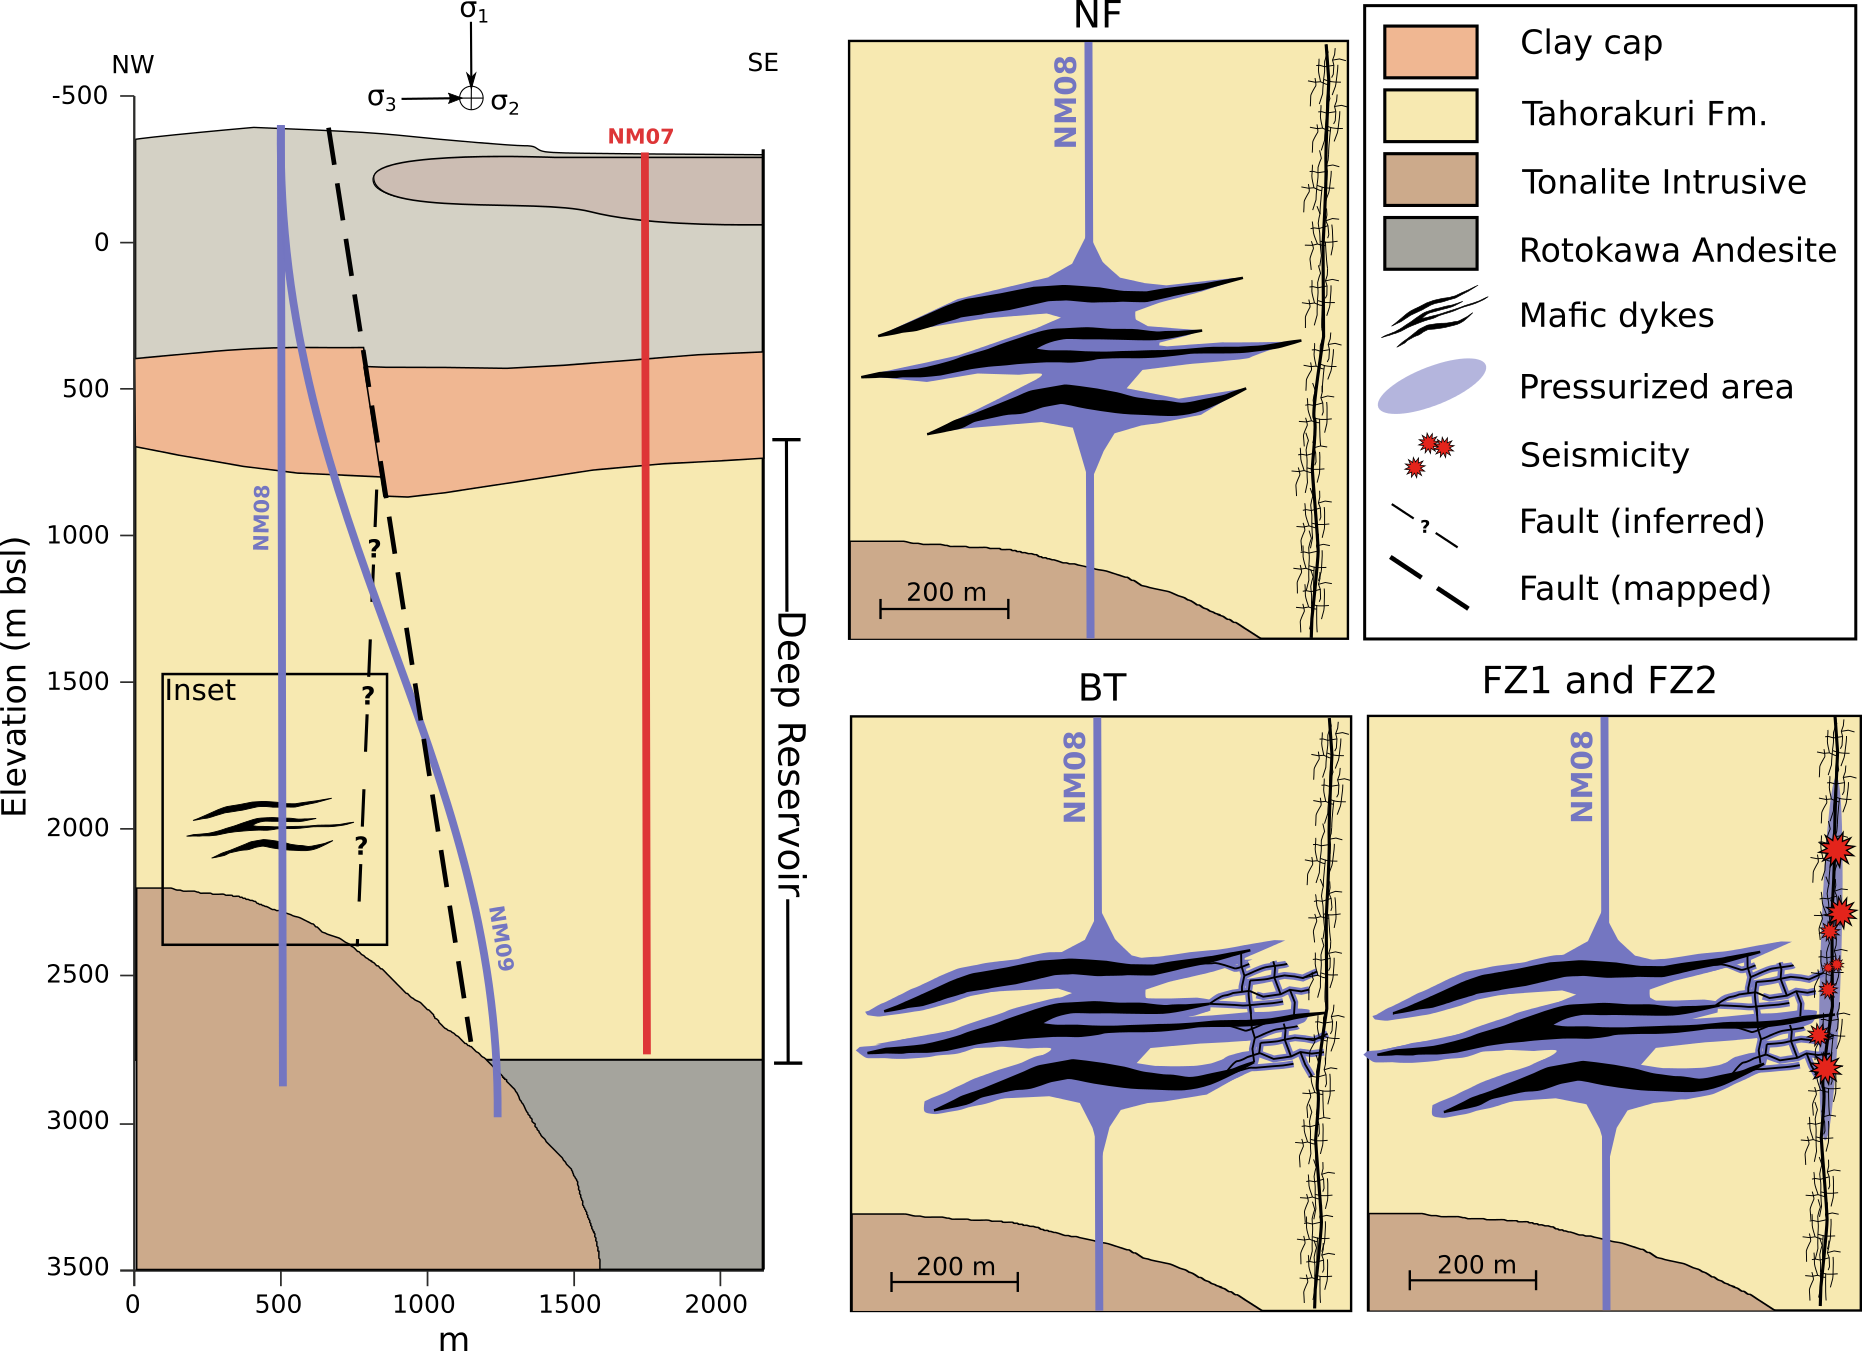
\includegraphics[width=1.00\columnwidth]{Chapter_3_Nga/figures/NM08_stimulation_cartoon/NM08_stimulation_cartoon_original}
\caption{{Schematic illustrating the sequence of events occurring at depth during
NM08 stimulation. The headings of the inset panels correspond to the
periods labeled at the top of Figure~{\ref{645772}}.
The main permeable zone in well NM08 corresponds to a depth where the
well intersects a mafic dike swarm. During NF, hydraulic conductivity
between NM08 and the soon-to-be-active fracture zone was low. This
period corresponds to a pressurization of the small, near-well fracture
network hosted in and around a set of mafic dikes, hence the relatively
high WHP but lack of seismicity. During BT, while WHP was below 2 MPa, a
hydraulic connection was established with the fracture zone, consistent
with increasing injectivity at the well. During FZ1, once WHP was
increased to a steady 2 MPa, the pressure perturbation was able to
diffuse into the fracture zone, weaken suitably oriented fractures and
generate seismicity. At the start of phase two, the fracture network
repressurized until it reached the maximum pressure encountered during
phase one, at which point seismicity recommenced (FZ2).
{\label{740510}}%
}}
\end{center}
\end{figure}

\subsubsection{NM09 injection testing}
Injection well NM09, in the north of the field, underwent two periods of injection prior to plant startup (supplements), accepting $\sim$56,000 m$^3$ of water between 13 December, 2012 and 4 January, 2013 and $\sim$60,000 m$^3$ of geothermal brine between 12 February and 6 March, 2013. The second of these tests used geothermal fluid injected directly from the plant ($\sim$90\textdegree{C}), and not river water ($\sim$10--20\textdegree{C}) as was injected at NM08, meaning that the degree of thermal contraction of the near-wellbore fracture walls was likely less than during the first portion of the NM09 test or at NM08. If we perform the same calculation for circumferential (hoop) stress as done previously for NM08, but with a $\Delta{T}$ of 120\textdegree C, instead of 204\textdegree, we get a thermally-induced stress of --32 MPa, or $\sim$60 \% of the stress induced by cold-water stimulation. Only 11 seismic events were detected within the reservoir during both phases of NM09 stimulation combined. Given that NM08 and NM09 were drilled in the same part of the reservoir, the difference in seismic response is surprising. However, \citet{Clearwater_2015} pointed out that there are major structural differences between NM09 and NM08, despite their proximity. NM08 was drilled directly into the low-permeability intrusive body in this section of the field, whereas NM09 is deviated and was completed in the intrusive's highly-permeable damage zone. Importantly, image logs reveal that NM09 intersects a number of highly-permeable fault zones at depths of $\sim$1850--2300 m bsl \citep{nm09_report}, which were not intersected by NM08. During reservoir tracer testing, it was also shown that NM09 is better-connected to the production wells than NM08 \citep{buscarlet_2015}. This implies a degree of compartmentalization in the northern reservoir, with the structure delineated by the NM08 seismicity possibly acting as a cross-strike flow barrier \citep{buscarlet_2015} (Figure \ref{532034}).

The high-permeability feedzones at NM09 inhibit pressure buildup in the reservoir during injection. During the injection tests, WHP at NM09 never exceeded 0.1 MPa and was often zero, implying that fluid entered the reservoir under its own weight, thereby decreasing the likelihood of inducing seismicity through pore-pressure diffusion. However, injectivity increased in the absence of seismic slip (n=$\sim$0.4--0.6) \citep{Clearwater_2015}. As at NM08, this observation indicates that permeability was enhanced through undetected (small) seismic slip, aseismic slip\slash{opening} of permeable zones connected to the wellbore, or both. It also reveals an even stronger decoupling of injectivity and near-well seismicity than at NM08, with the observed gain likely a result of thermoelastic stresses near the wellbore, especially during cold water injection in phase one.\selectlanguage{english}
\begin{figure}[h!]
\begin{center}
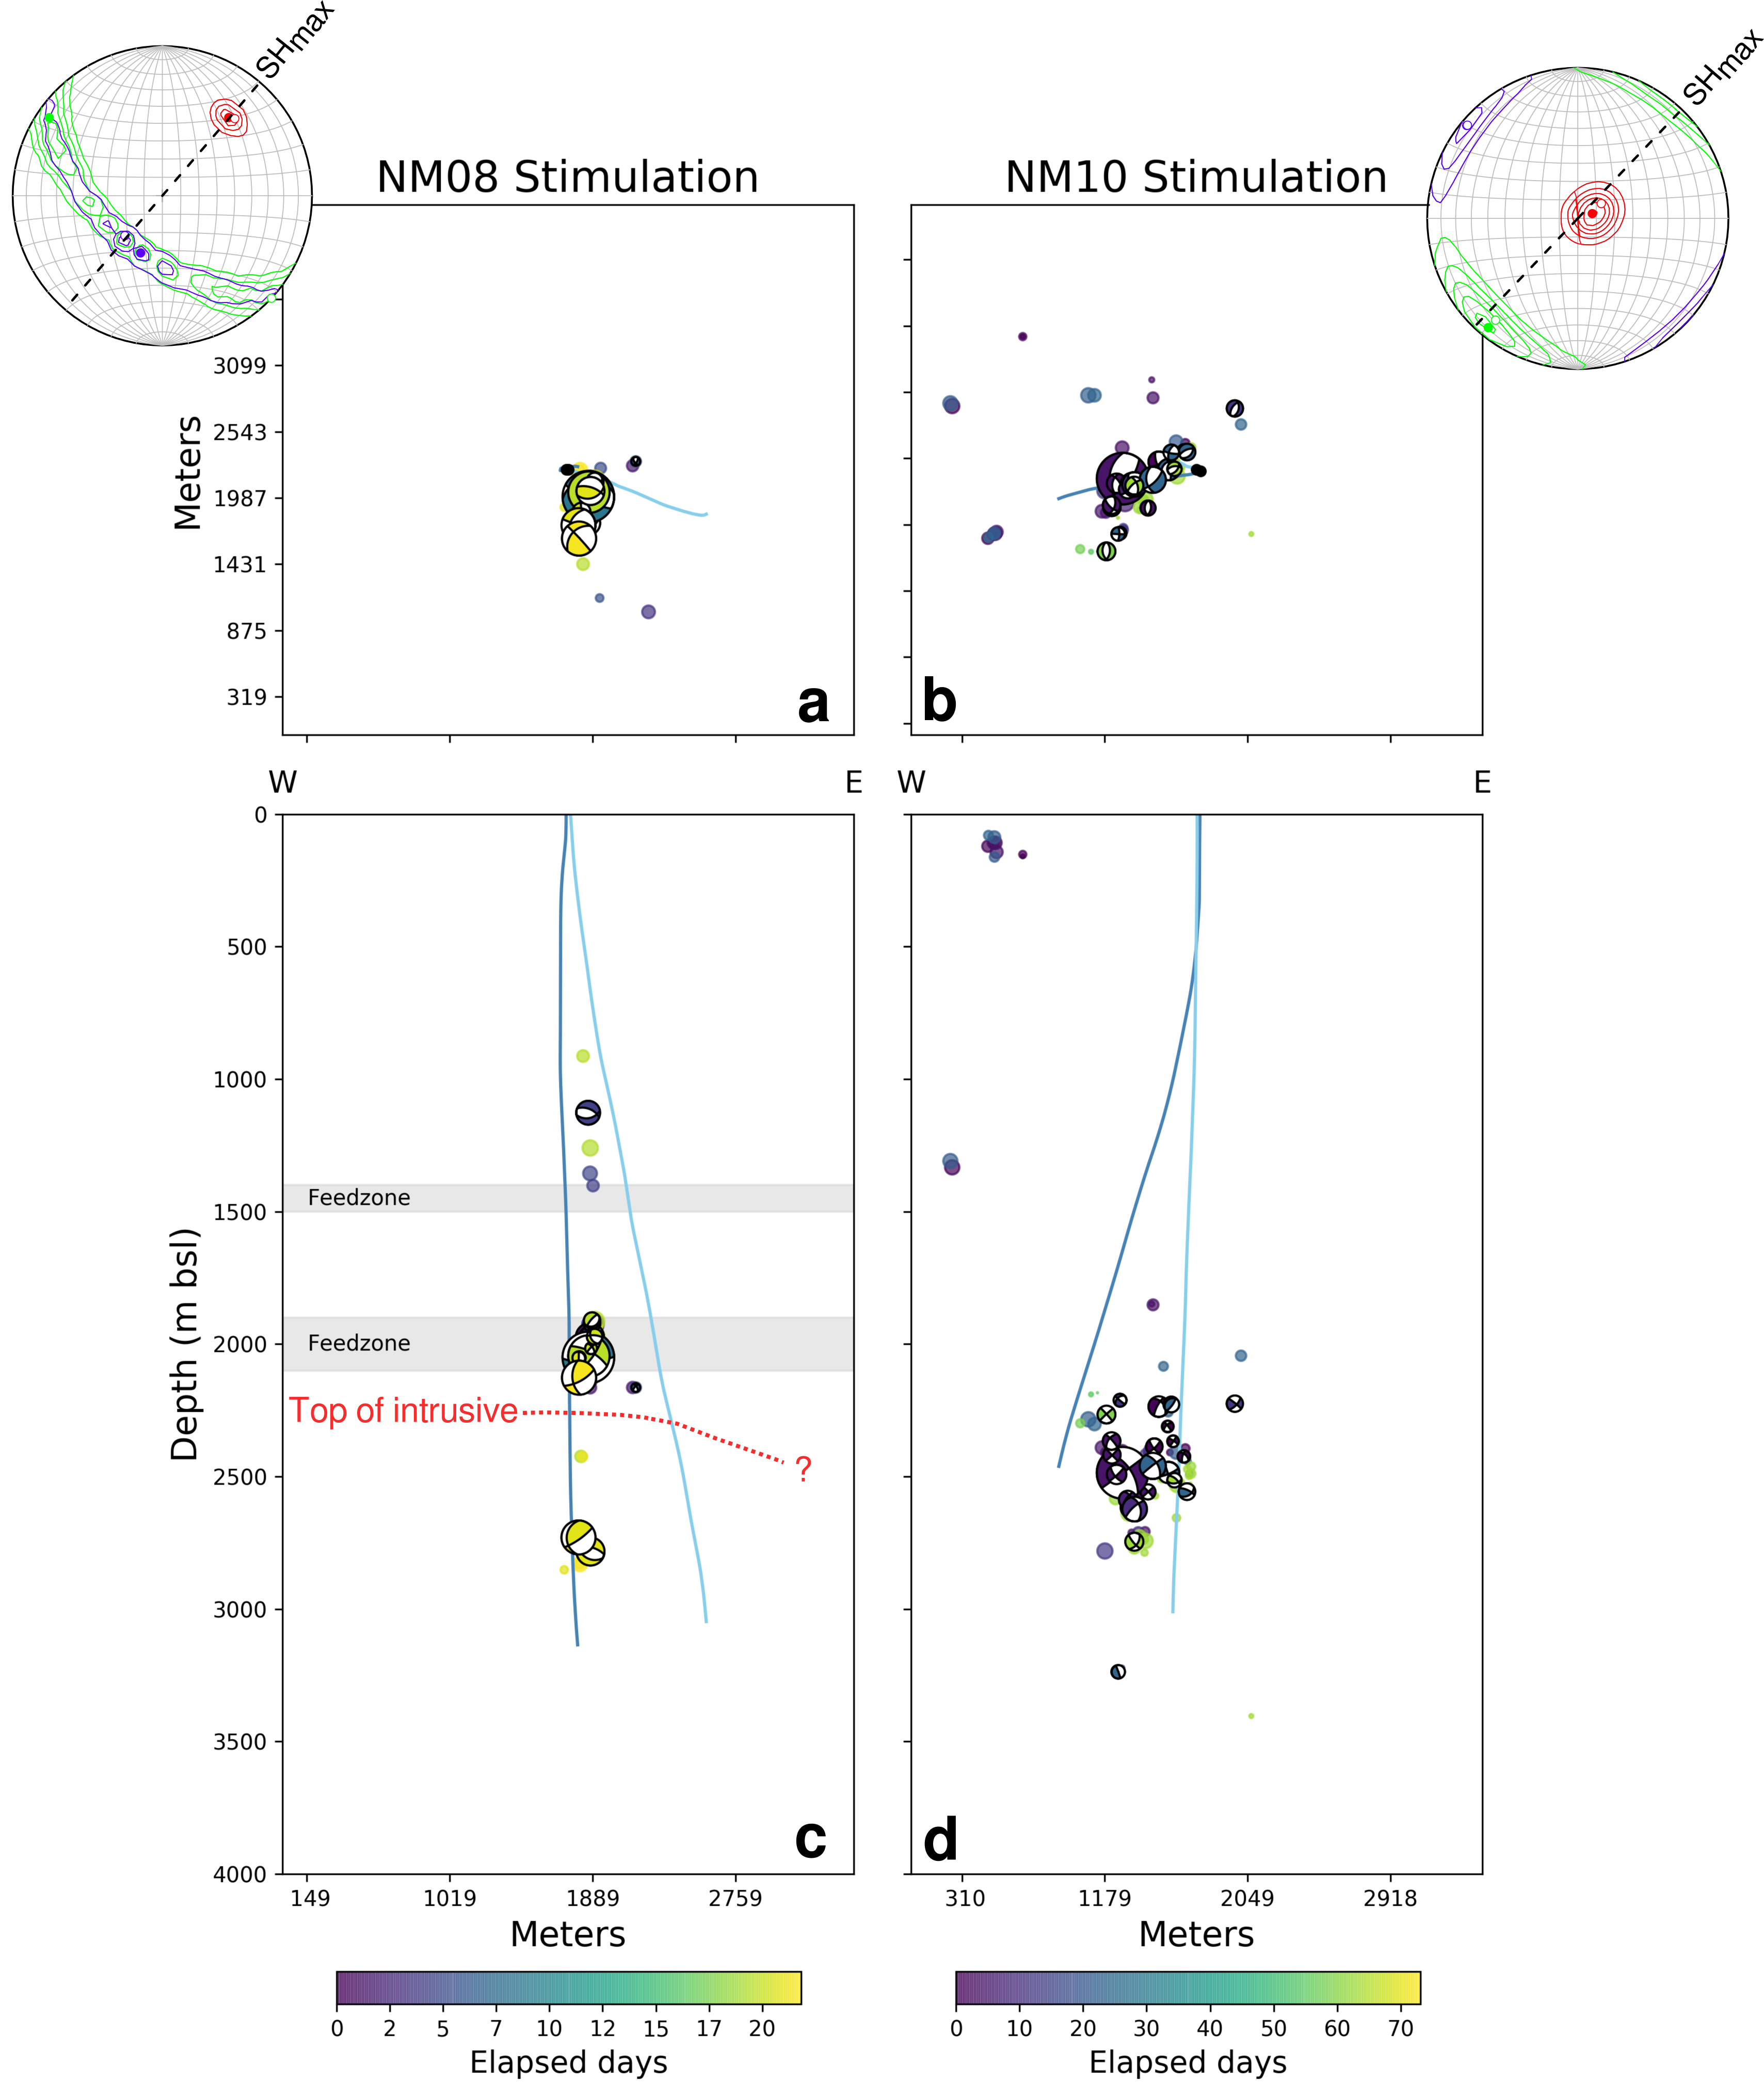
\includegraphics[width=0.84\columnwidth]{Chapter_3_Nga/figures/Nga_stims_map_depth_beachballs_stress_final_labels_10-5_intrusive_colored/Nga_stims_map_depth_beachballs_stress_GC_labels_12-5_intrusive_colored_dpi300_original}
\caption{{P-wave first-motion-derived focal mechanisms for template events which
occurred during various phases of injection testing at Ngatamariki. Dark
blue mechanisms in a and c occurred during stimulation of NM08, in the
northern injection zone. Green mechanisms occurred during NM10 drilling
losses and injection testing (panels b and d; southern zone). The
symbols plotted in cross-sections c and d have been reprojected to
reflect the different viewpoint (from the south). The inset figures in a
and b show stress inversion results (lower hemisphere) from the focal
mechanisms presented in northern and southern Ngatamariki, respectively,
with red contours representing the probability density of the direction
of~\(\sigma_1\), green representing~\(\sigma_2\) and blue
representing~\(\sigma_3\) . The black dashed line indicates the
direction of SHmax. In panel c, the red dashed line indicates the top of
the intrusive sequence in northern Ngatamariki. As the extent of this
unit is only constrained by core from wells NM04 (northeast of panel a),
NM08 and NM09, its shape, volume and orientation are unknown.
{\label{532034}}%
}}
\end{center}
\end{figure}

\subsection{Southern Injection Zone}
\subsubsection{NM10 drilling losses and injection testing}
Well NM06 was drilled and tested in the southern injection zone, many years prior to our study. As a result, drilling and well testing in southern Ngatamariki during this study period was limited to injection well NM10. Injection began once drilling had reached the depth of the deep (andesite) reservoir and drilling-fluid losses occurred (at depths \textgreater2000 m bsl). This was followed by a formal injection\slash{stimulation} test once drilling had been completed. The microseismic response to the drilling losses was larger than the response during the actual injection test (Figures \ref{703798} \& \ref{640752}). At the end of drilling, approximately 57,000 m$^{3}$ of drilling fluid (largely water) had been lost to the formation, a comparable volume to that in the other injection tests analyzed and described above. Data on fluid flow during drilling are sampled less frequently than the flow rate data during injection tests, but daily records of drilling losses correlate well with seismicity in southern Ngatamariki as shown in Figure \ref{703798}a. NM10 drilling reached 1700 m bsl on 6 July 2012 and significant fluid losses were incurred from 13 July ($\sim$2100 m bsl).

Seismicity began as the drilling reached the depth of a major fault zone identified in the NM10 image logs (there are six identified faults between 2100 and 2300 m bsl, within the Rotokawa Andesite \cite{nm10_report}) and continued for the remainder of the drilling (Figure \ref{703798}c). These SE-dipping structures, visible in image logs \citep{nm10_report}, are likely associated with the NE--SW-striking Aratiatia Fault Zone (Figure \ref{795275}, \ref{827409}, \ref{532034}). Seismicity increased in short, 1--2 day-long bursts with the majority of events occurring after fluid losses had exceeded 25 t/h. The lag between the start of fluid losses and the seismicity induced during NM10 drilling is roughly three days, three times shorter than at NM08. This lag may simply be due to the time needed to pressurize the fault zones, which dominate flow from NM10. However, aseismic opening of the fault zones via pore-pressure increase and thermal contraction of the fracture walls, as observed by \citet{Guglielmi_2015}, may also have played a part. We would expect these processes to be accompanied by a corresponding increase in injectivity, but there are no pressure data during the drilling to confirm this. The seismicity occurred \textgreater700 m deeper than the main feedzones in NM10 (Figure \ref{827409}), and closer to injection well NM06, which was shut-in during this period. This may indicate that fluid flowed down-dip along the fault zone to critically stressed points away from the well. The maximum magnitude during drilling at NM10 was 2.1, comparable to the stimulation at NM08 for a similar injected volume. This may indicate that the pressurized zones during NM08 stimulation and NM10 drilling were similar in volume, thereby affecting fractures and faults of similar size. However, as southern Ngatamariki exhibits a lower b-value than in the north when the entire four-year catalog is taken into account, we suggest that much larger structures exist in the south than the north, which were only activated once high-volume injection began in 2013. As at NM08, seismicity ceased after end of drilling implying that the permeability of the fracture zone is considerable.\selectlanguage{english}

\begin{figure}[h!]
\begin{center}
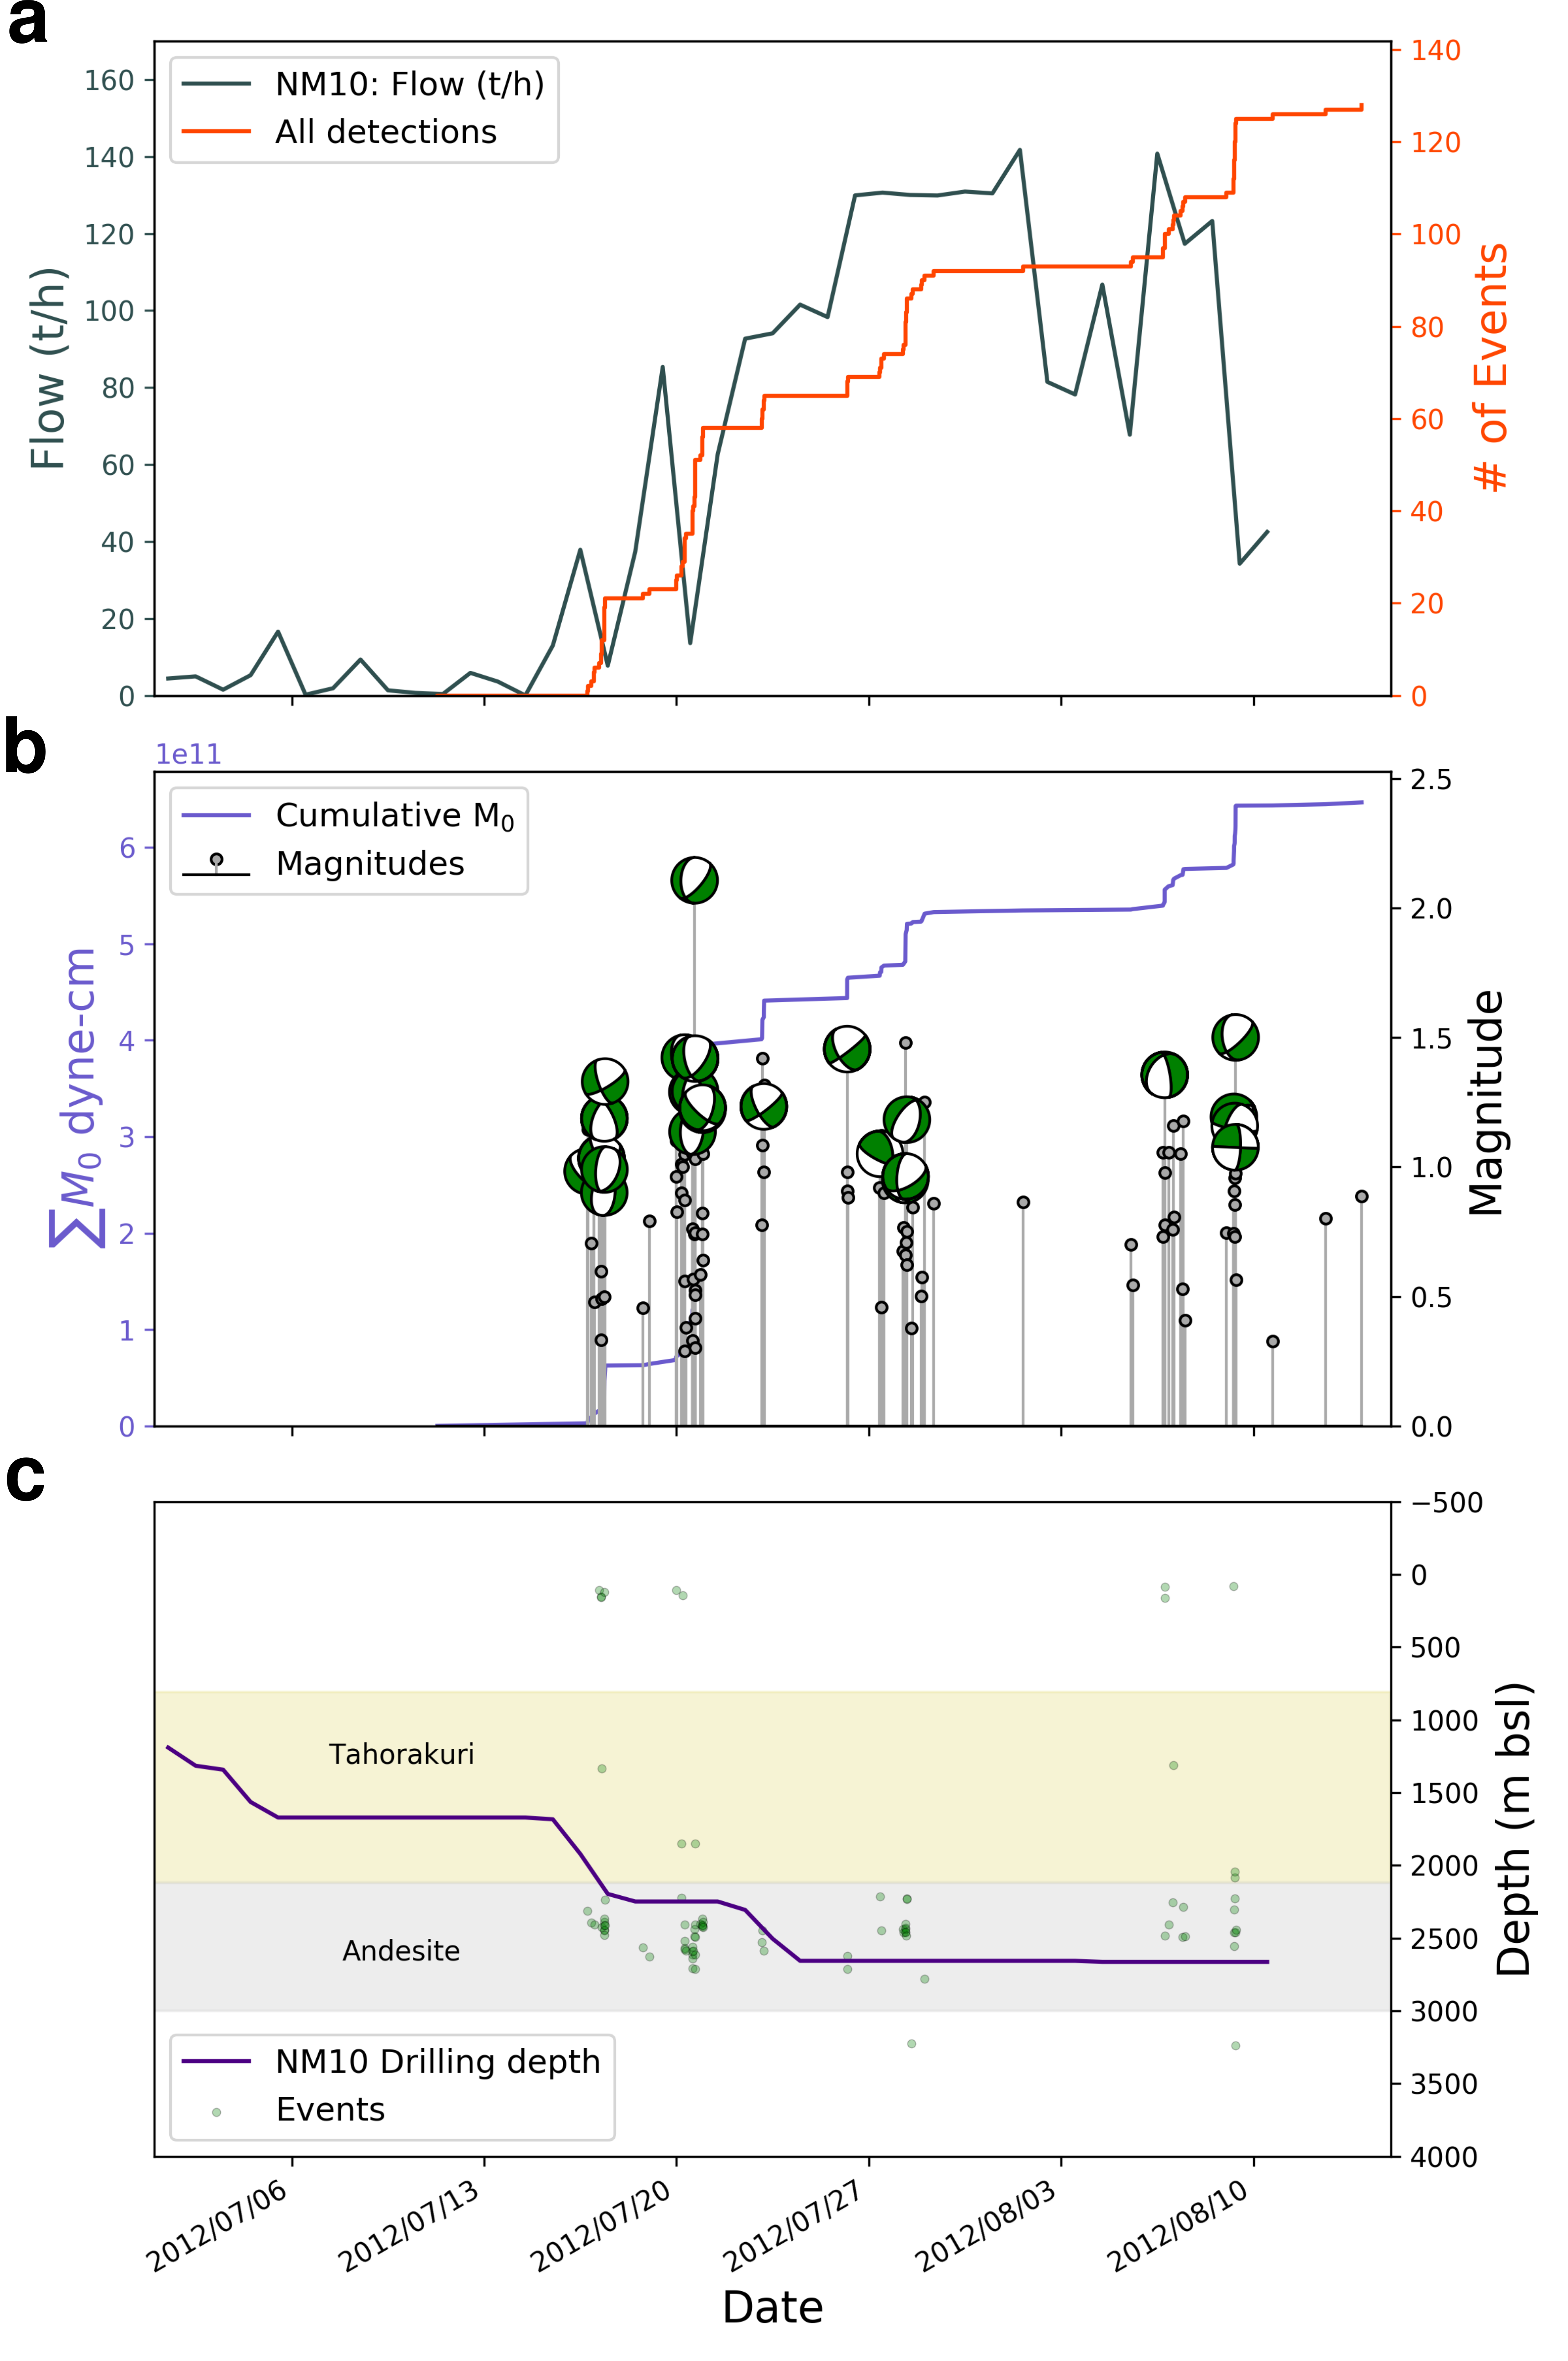
\includegraphics[width=0.84\columnwidth]{Chapter_3_Nga/figures/Multiplet_150_vs_flow_cum_NM10_losses/Full_final_cat_flow_mags_FMs_depth_NM10_Drilling_12-5_GrowClust_no_diff_ABC_original}
\caption{{a) Flow (t/h) during fluid losses and cumulative seismicity vs time, b)
cumulative seismic moment with event local magnitudes and available
focal mechanisms during drilling of NM10 and c) drilling depth with
depth of seismic events. The two main geological units within the
southern reservoir, the Tahorakuri Volcaniclastics and Rotokawa
Andesite, are depicted in c) for context.
{\label{703798}}%
}}
\end{center}
\end{figure}

There were no drilling or injection activities in southern Ngatamariki between the drilling of NM10 and the planned injection test that occurred on 1--23 September, 2012. There was also no detected seismicity during this period. Roughly 73,000 m$^3$ of fluid was injected during the test at flow rates of between 100 and 200 t/h and downhole pressures of 7.5--9.4 MPa (Figure \ref{640752}). As mentioned above, the unintended losses that occurred during drilling are considered the start of injection in southern Ngatamariki. Therefore, during drilling, NM10 may have undergone much of the increase in injectivity that otherwise would have occurred during the later injection test. It is possible that slip during drilling relieved most of the accumulated stress on the most critically stressed portions of the fault zone, making failure on these patches less likely during the injection test. This view is supported by the relative lack of seismicity during most of the test (Figure \ref{640752}). Seismicity, while not absent, occurred for the first two weeks of the test at a rate of roughly one event per day, and injectivity increased only slightly after the first step-rate change in flow from $\sim$100 to 150 t/h. However, the rate of seismicity jumped dramatically (with nearly 40 events on 17 September alone) once injection was increased from $\sim$150 t/h to $\sim$200 t/h. We do not know the corresponding increase in downhole pressure for this step-rate change because the pressure monitoring tubing was repositioned at that time. However, because the flow rate of 200 t/h is significantly higher than was measured during either drilling or testing prior to this time, we can reasonably assume that the downhole pressure would have increased beyond any previously-recorded level at NM10, and therefore would be expected to induce seismicity (again due to the `Kaiser effect' \citep{Holcomb_1993}). The resulting increase in the rate of seismicity occurred within two hours of the increase in flow rate and at event--feedzone distances of up to 800 m (Figure \ref{640752}a and \ref{640752}b). As during FZ2 at NM08, inducing events at such distances so rapidly requires that pressure change be concentrated along a small number of highly-permeable fracture zones, which is what we expect in NM10 on the basis of image logs. Once flow rate had subsided to below 200 t/h, seismicity ceased, suggesting rapid progression of the back-front to the seismically active zone as was observed at NM08. The maximum magnitude during the injection testing of NM10 was 1.4, lower than during NM10 drilling, possibly as a result of the stress acting on the fracture zone having been relived during drilling fluid losses.\selectlanguage{english}

\begin{figure}[h!]
\begin{center}
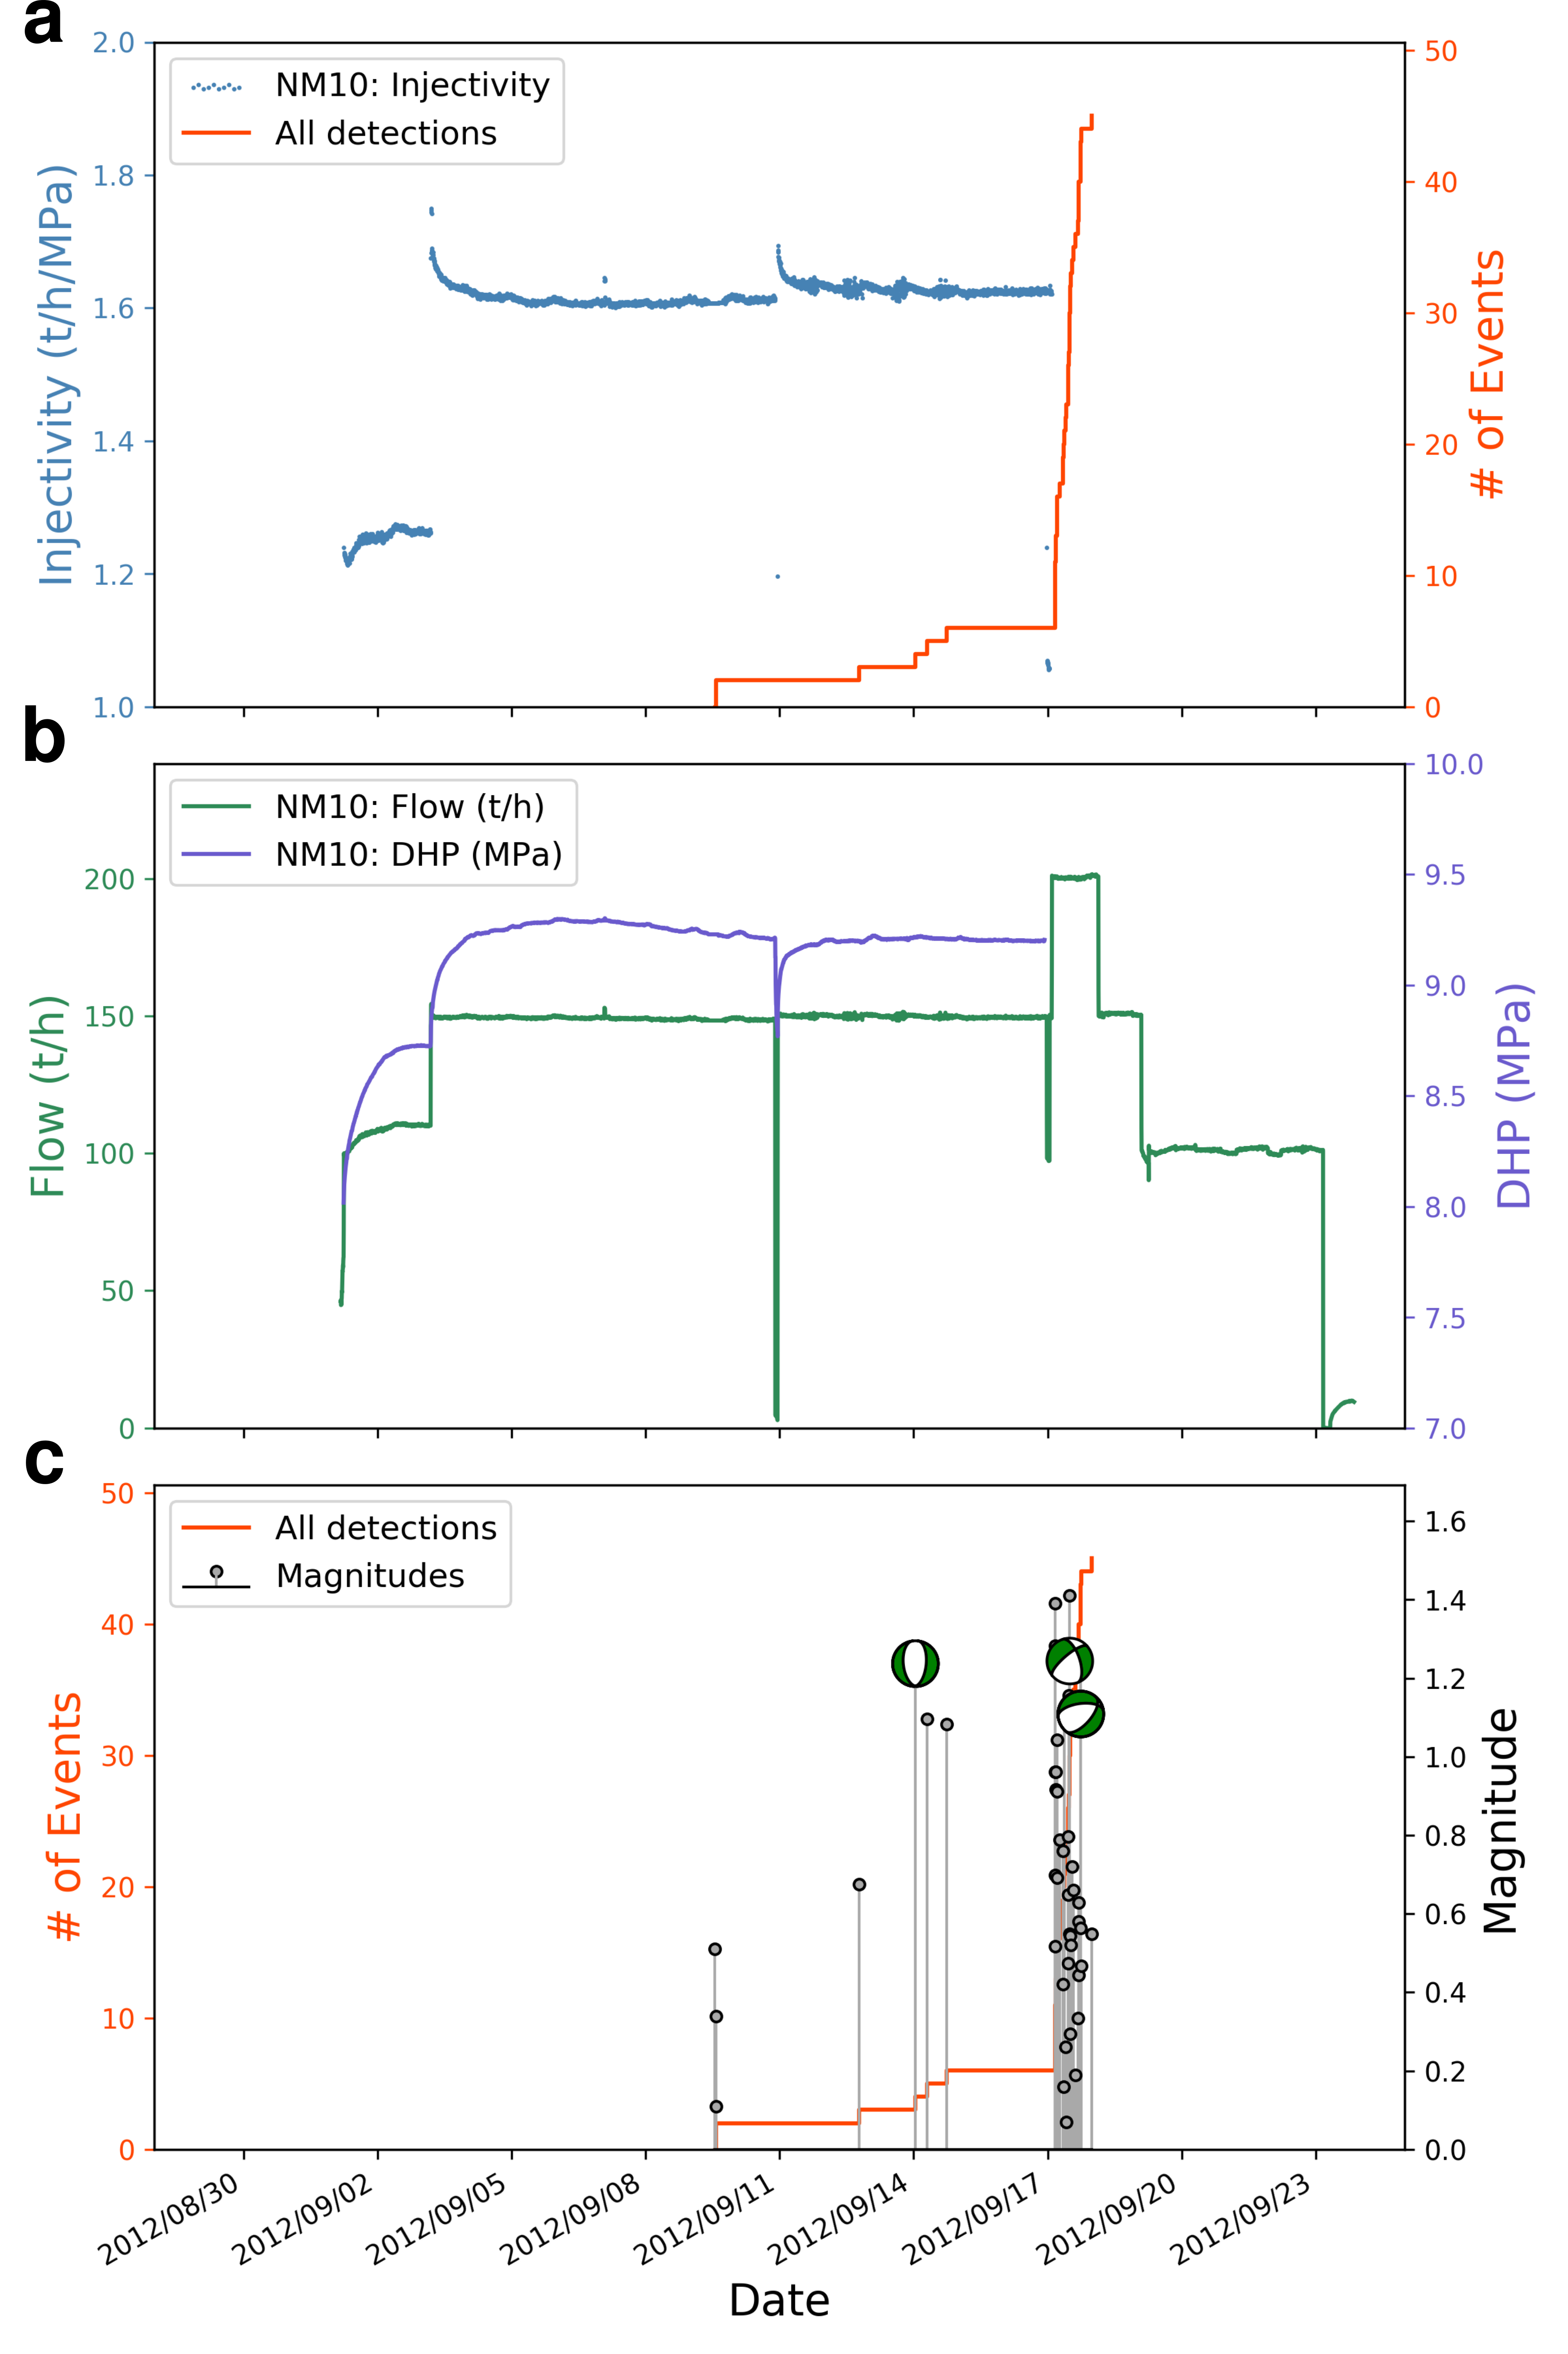
\includegraphics[width=0.84\columnwidth]{Chapter_3_Nga/figures/Multiplet_150_vs_flow_cum_NM10_stim/Full_final_cat_flow_mags_FMs_depth_NM10_Stimulation_12-5_GrowClust_labels_no_diff_ABC_original.png}
\caption{{a) NM10 injection test II vs. cumulative seismicity in southern
Ngatamariki, b) Flow rate and downhole pressure. DHP ends on 17 Sept as
the measurement tubing was traversed to a greater depth (from 1228 m to
2050 m). c) Cumulative seismicity in red with the magnitude and
available focal mechanism solutions as stems.
{\label{640752}}%
}}
\end{center}
\end{figure}

\subsection{Focal mechanisms and stress}
Figure \ref{532034} shows the focal mechanisms calculated for microearthquakes that occurred during the three well injection tests described above, and the corresponding stress inversion results for northern and southern Ngatamariki prior to plant startup. The events that occurred during drilling and injection testing of NM10 (Figure \ref{532034}b and d) delineate a structure associated with the Aratiatia Fault Zone, as mentioned above. The majority of the 28 focal mechanisms we calculated for southern Ngatamariki during this time period show predominantly normal faulting, with most fault planes striking N--S or NE--SW. This result agrees well with what is known about the extensional regional stress regime and the local faults in the central TVZ, which are typically oriented NE--SW \citep{Massiot_2015}. Acoustic- and resistivity-based image logs for NM10 confirm this preferred NE--SW fracture orientation at reservoir depths with predominantly SE dips \citep{nm10_report}. As mentioned in Sections \ref{Plant_ops} and \ref{location_results}, rapid injection returns during a tracer test conducted in January 2014 also indicate that a highly permeable flow pathway connects NM10 to production well NM05 \citep{buscarlet_2015}. The locations of the events induced during NM10 drilling and injection testing are likely related to fluid flow along this structure.

Stress inversion results for southern Ngatamariki (inset, Figure \ref{532034}b) show $\sigma_1$ to be subvertical and the direction of maximum horizontal compressive stress ($S_{HMAX}$) to be NE--SW, consistent with previous findings for the central TVZ \citep{Townend_2012} as well as measurements of borehole breakout in NM10 which indicate an $S_{HMAX}$ azimuth of 210\textdegree \citep{nm10_report}. This result is also consistent with breakout measurements from the Rotokawa geothermal field, 5 km to the south \citep{McNamara_2015}.

The 58 blue mechanisms in Figure \ref{532034}a and c correspond to events that occurred during the stimulation of NM08 and exhibit a greater variety of faulting kinematics than in the south. Many of these mechanisms show primarily reverse or oblique strike-slip movement with at least one nodal plane striking NW--SE, which agrees with the orientation of the plane defined by the hypocenters of the events (strike 192\textdegree, dip $\sim$66\textdegree). The remaining mechanisms show normal faulting with a variety of strikes. The occurrence of compressional faulting is rare within the central TVZ and may be related to stress field rotation during the emplacement of the intrusive body and mafic dikes.

Stress inversion results for northern Ngatamariki differ from those in the south (insets in Figure \ref{532034}a and b). While the direction of $S_{HMAX}$ is unchanged throughout the reservoir (NE--SW), $\sigma_1$ is dipping NE at approximately 30\textdegree{} in the north and $\sigma_2$ and $\sigma_3$ define a girdle. It is possible that the stress state in this section of the reservoir was already rotated into an orientation suitable for reverse faulting by the emplacement of the tonalite intrusive body and dikes. \citet{massiot_2012} showed that the in-situ horizontal stress field rotates counter-clockwise by 28\textdegree{} near the contact between the Tahorakuri and the intrusive body (below the main permeable zone and dikes, relative to the stress field above), which may indicate an intrusive-related effect on the stress state.

What is not known is the effect of injection-related pressure buildup and thermoelastic stresses on the stress in the reservoir (Figure \ref{111394}). We have no DHP measurements during stimulation of NM08. However, wellhead pressure reached 2.6 MPa during the near-field period of stimulation (NF, Figure \ref{645772}). Figure \ref{111394}a shows the destabilizing effect of pore pressure increase on the reservoir stress state, with the increase in P$_f$ exaggerated for visibility. We infer that the fracture zone defined by the seismicity during NM08 stimulation is nearly-critically-stressed within the reservoir stress regime and would require only small increases in pore pressure to induce slip (blue and red circles, Figure \ref{111394}a).

Circumferential stresses reached roughly -54 MPa at the wellbore (at 2000 m bsl), but it is difficult to determine how far such thermoelastic effects would propagate from the well as the propagation of the thermal front is dependent upon the flow pathways and flow rate through the reservoir. During a stimulation operation at the naturally-fractured Geysers geothermal field, \citet{Jeanne_2015tensor} modeled a similar thermal front propagating \textgreater100 m in the span of two months. For a reservoir where fluid flow is fracture dominated, the corresponding cooling effect depends on the predominant direction of flow relative to the principle stress axes, as illustrated in Figure \ref{111394}b \citep{Jeanne_2015tensor}. This is because the rock matrix is cooled conductively only within \textless1 m along the normal to a fracture plane, whereas it is cooled for many tens of meters along the strike of a fracture, leading to an anisotropic volume of thermal cooling \citep{De_Simone_2013,Jeanne_2015tensor}. Initial, gravity-driven (downward) flow of cool fluid at NM08 would preferentially decrease $\sigma_{1}$ and stabilize the near-well fracture network (yellow Mohr circle, Figure \ref{111394}b). This may have contributed to the lack of seismicity during the NF and BT periods of NM08 stimulation (Figures \ref{645772} and \ref{740510}). As fluid begins to spread laterally from the well, the cooling effect preferentially lowers the horizontal stress that is best aligned with the direction of flow. At Ngatamariki, fluid flow parallel to $\sigma_{3}$ (NW--SE) would act to destabilize the fracture network (pink Mohr circle, Figure \ref{111394}b), including the structure along which seismicity occurred, which is represented as a colored circle for the various stress fields illustrated in Figure \ref{111394}.

As the Ngatamariki reservoir is structurally similar to that of the Geysers, in that they are both naturally-fractured, high-temperature fields, it is possible that a thermoelastic front could have reached the location of seismicity during stimulation of NM08 and therefore influenced the stress state in the fracture zone. Also at the Geysers, \citet{Mart_nez_Garz_n_2013} observed temporal changes in focal mechanism-derived stress tensors related to various fluid injection operations (including the injection operation modeled by \citet{Jeanne_2015tensor}), although this contrasts with the findings of \citet{Boyle_2014} who found that operations at the Geysers had little effect on the reservoir stress state. We cannot rule out the possibility that the deviation of the stress field from the regional trend in northern Ngatamariki is injection-related, although we think it unlikely. As discussed above, it is also possible that the stress state was already rotated in the northern injection zone prior to injection.\selectlanguage{english}

\begin{figure}[h!]
\begin{center}
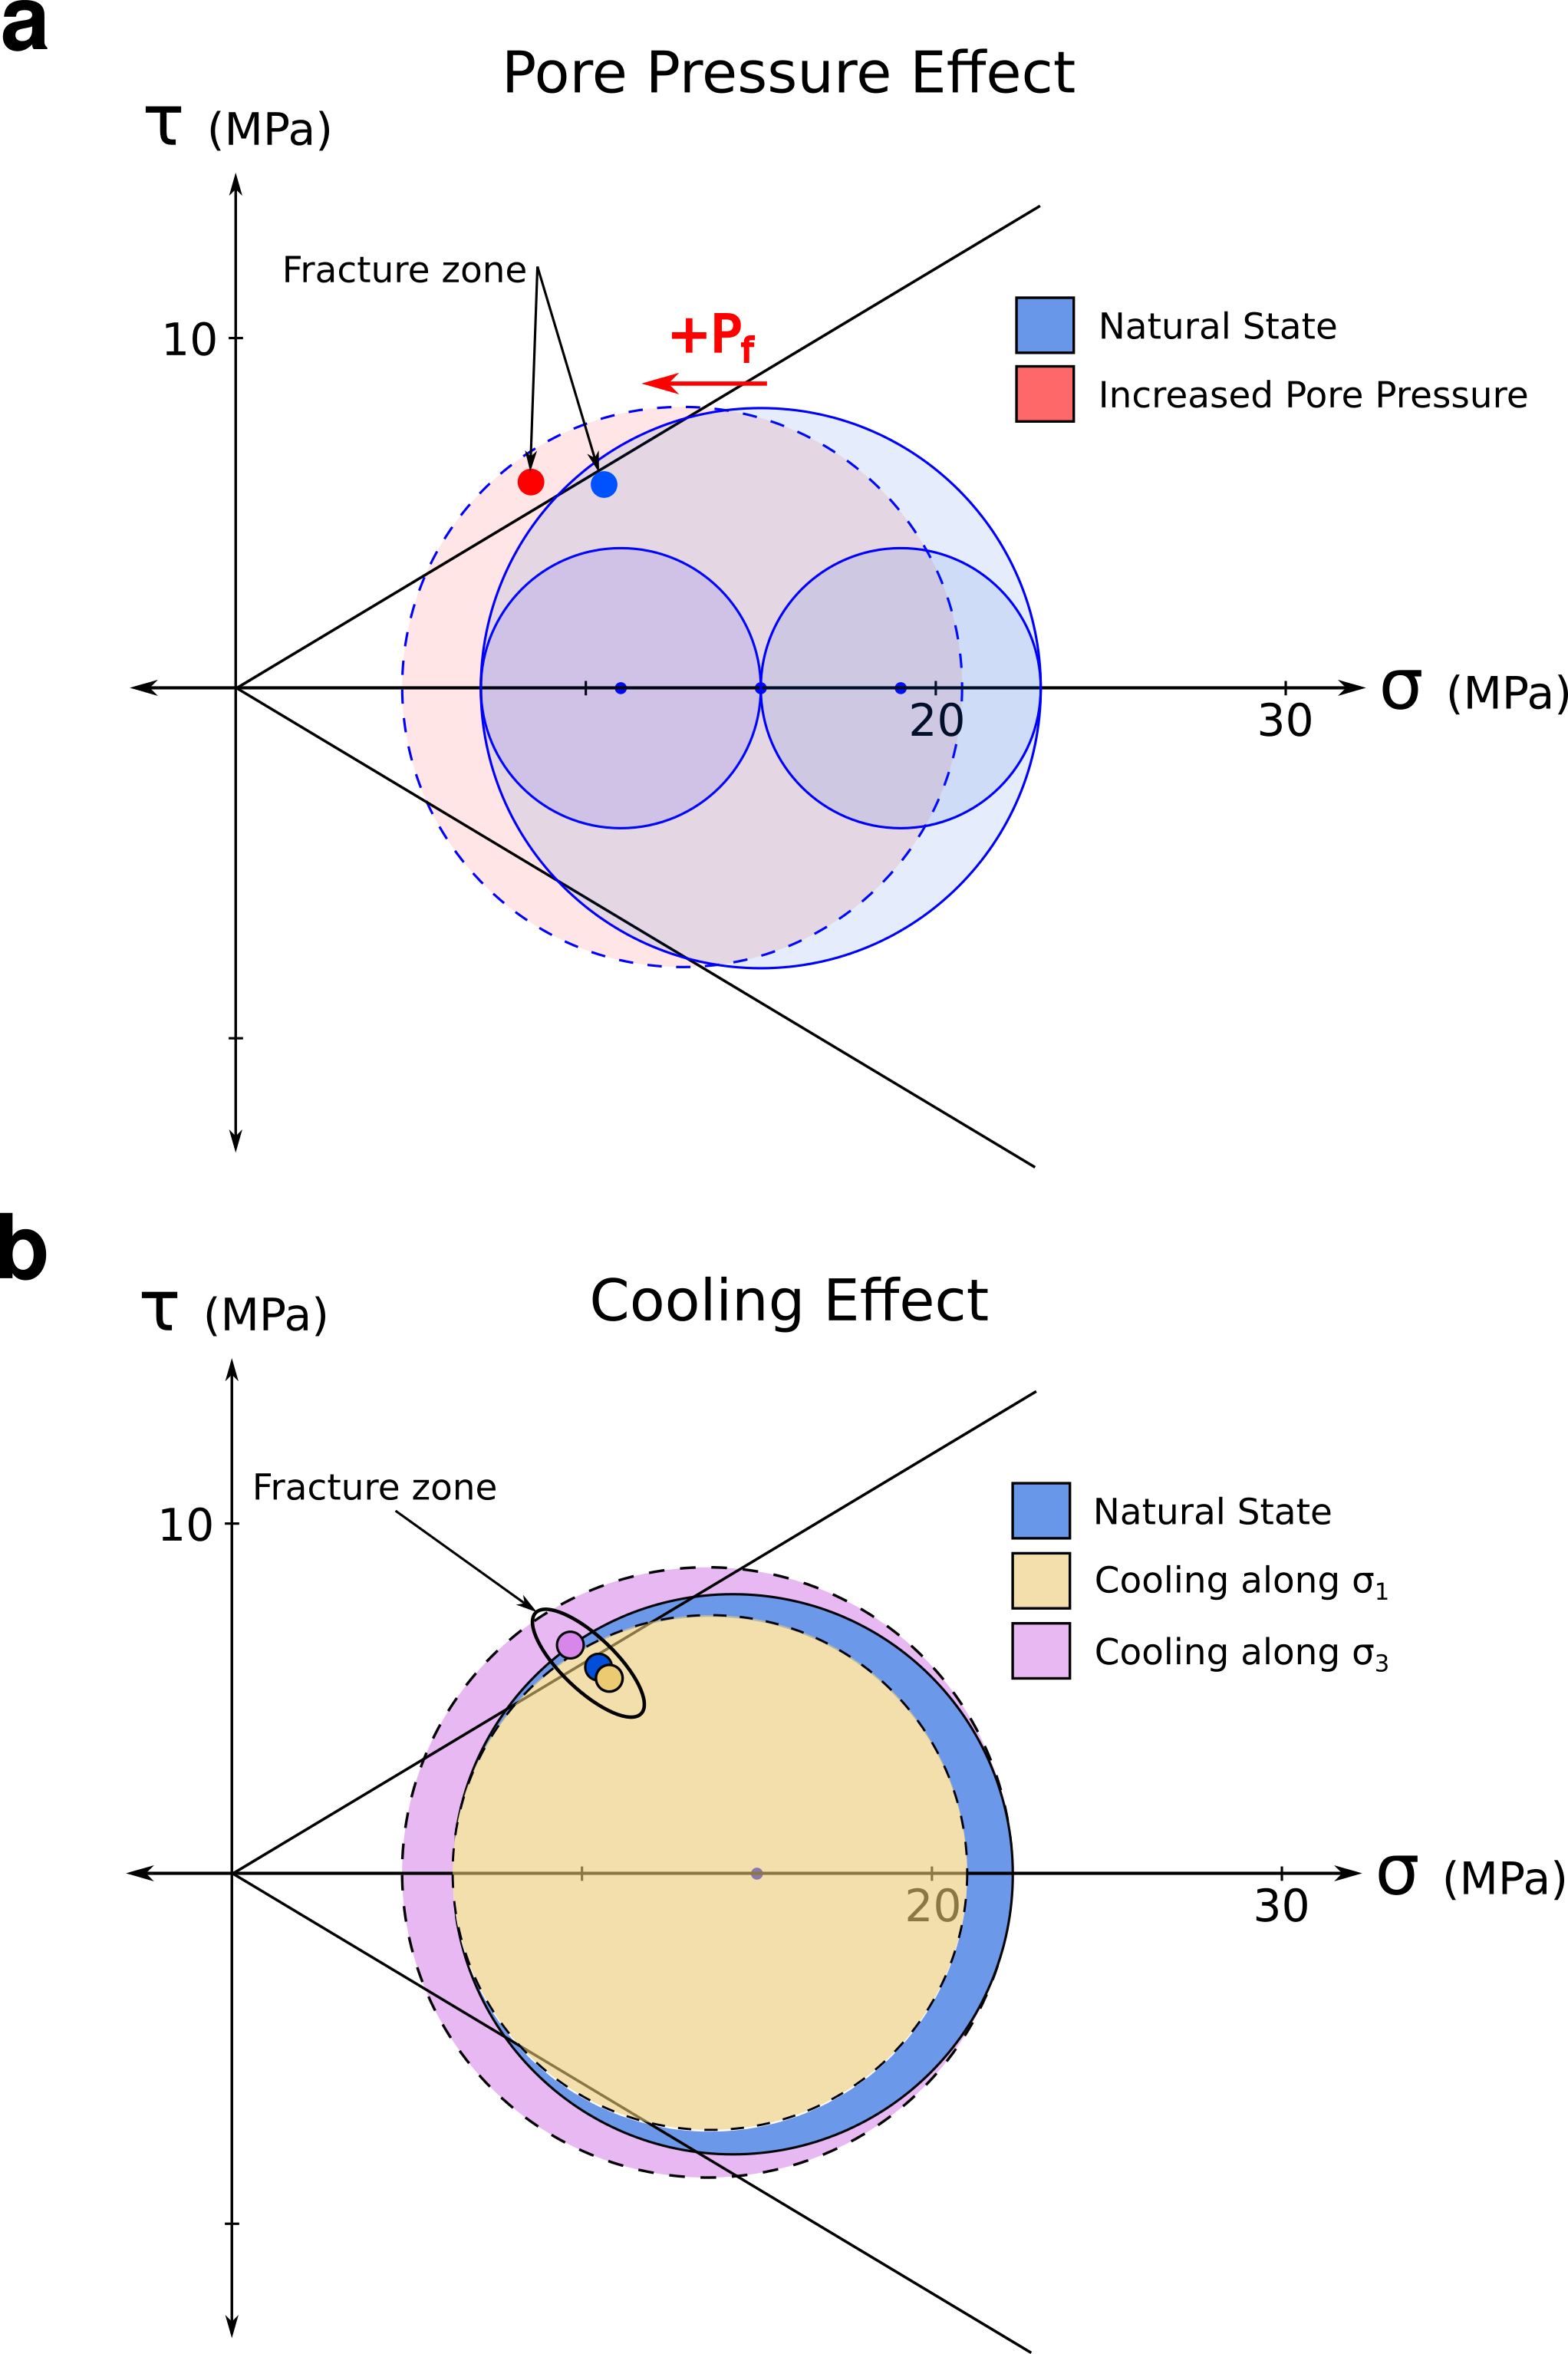
\includegraphics[width=0.70\columnwidth]{Chapter_3_Nga/figures/Nga_2000mbsl_NM08_fz_schematic/Nga_2000mbsl_NM08_fz_schematic_original.png}
\caption{{Schematic Mohr circles calculated for a depth of 2000 m bsl illustrating
the effect of a) pore pressure increase and b) thermal cooling of the
fracture zone near well NM08 (strike: 191\textsuperscript{o}, dip:
66\textsuperscript{o}). The natural state magnitude
for~\(\sigma_{1}\) was determined by integrating density over depth
using density values from well cuttings and core taken from NM08
($\sim$45 MPa at 2000 ms). The magnitude
of~\(\sigma_{3}\) was extrapolated from leak-off tests conducted in
Rotokawa ($\sim$29 MPa)~\protect\citep{davidson_2012}. Reservoir
pressure is approximately 22 MPa at 2000 m bsl. The failure envelopes
represent cohesionless, preexisiting fractures with a coefficient of
friction of 0.6. Circles in the figure represent the position of the
plane defined by the hypocenters of seismicity during NM08 stimulation
within each stress field. Plots are adapted from the output
of~\href{http://www.geo.cornell.edu/geology/faculty/RWA/programs/mohrplotter.html}{MohrPlotter}~\protect\citep{Allmendinger}.
{\label{111394}}%
}}
\end{center}
\end{figure}

\section{Conclusions}
Ngatamariki constitutes an important case study of isolated injection into a little-modified reservoir. In this paper we present a nearly four-year catalog of microearthquakes at the Ngatamariki geothermal field spanning periods of initial field development, well drilling and plant startup. Individual tests at each well were isolated from one another in both time and space, which has allowed us to observe the response of microseismicity to injection at individual wells. Seismicity occurs in two spatial clusters centered on the northern and southern injection zones. In the north, stimulation of well NM08 induced more than 120 events in one month, while injection testing of nearby well NM09 generated only 11 events in nearly three months. In southern Ngatamariki, drilling and injection testing of NM10 generated nearly 200 events over an interval of roughly three months. The difference between the frequency-magnitude distributions of the northern and southern clusters provides a clear example of b-value dependence on the characteristics of the local fracture network. In the north, the fractures that are hydraulically connected to wells NM08 and NM09 are smaller than those in the south, where fluid is injected into a large, active fault zone. As a result, larger events are able to nucleate in the southern injection zone (b$=$1.20) than in the north (b$=$1.84), resulting in a lower b-value.

Focal mechanisms calculated for events that occurred during these injections show different faulting regimes in the northern and southern halves of Ngatamariki. During the stimulation of NM08, in the northern part of the field, focal mechanisms exhibited a wide range of faulting kinematics, most with at least one nodal plane consistent with the NNE--SSW trend in hypocenter locations and a stress state with $\sigma_{1}$ dipping 30\textdegree. In contrast, NE--SW-striking normal faulting mechanisms make up the bulk of events occurring in the south. We interpret this contrast to be related to the presence of the tonalite intrusive body encountered at the bottom of the wells in northern Ngatamariki, which likely modified the local stress field in such a way that reverse and strike-slip faulting could occur in close proximity. However, as has been modeled and inferred for the Geysers geothermal field, another high-temperature, naturally-fractured reservoir \citep{Mart_nez_Garz_n_2014,Jeanne_2015tensor}, injection-induced stress tensor changes are plausible at Ngatamariki.

Fluid injection-induced slip on nearby, suitably oriented fractures is commonly assumed to be the main mechanism responsible for well stimulation. In the Ngatamariki case, however, induced seismicity occurs independently of near-well permeability gain, suggesting that seismic slip and permeability gained through self-propping play a subsidiary role in well stimulation. During the cold-water stimulation test at NM08, injectivity increased rapidly from the start of injection with no apparent sensitivity to the onset of seismicity ten days later. During injection at NM09, the well was also stimulated but was accompanied by only 11 detected seismic events despite two separate injections totaling \textgreater100,000 m$^3$ of fluid. In the south, interpretation of the cold-water stimulation of well NM10 was complicated by fluid losses during drilling, which induced nearly 140 events but for which no injectivity data exist.

This apparent decoupling of induced seismicity and near-well permeability suggests that slow, aseismic processes dominate well stimulation at Ngatamariki, specifically, but also at other high-temperature, high-permeability geothermal reservoirs where thermo-elastic stresses may lead to fracture opening but not necessarily to seismic slip. Other recent studies have raised the possibility that permeability and seismicity need not be related for cases of induced seismicity \citep[e.g.][]{Guglielmi_2015, Riffault_2018} and the dataset we present here contributes to the documentation and understanding of this discrepancy.

The degree of decoupling may be a product of the combined high-permeability and high-temperature of the Ngatamariki reservoir. Lower-temperature resources will not exhibit similar degrees of thermal stimulation and lower-permeability reservoirs are subject to higher pore-pressure perturbations, thus increasing the likelihood of inducing seismicity. However, if permeability enhancement and seismicity are decoupled, as we have shown for Ngatamariki, it may be possible to design injection operations in similar settings elsewhere in order to achieve the desired permeability gain while limiting the number and magnitude of induced seismic events.

\section{Acknowledgments}
We thank the Rotokawa Joint Venture (Tauhara North No. 2 Trust \& Mercury NZ Limited) for the funding to conduct this research and for allowing us access to the data and permission to publish our findings. We also wish to acknowledge the contribution of high-performance computing facilities to the results of this research. New Zealand's national facilities are provided by the NZ eScience Infrastructure (NeSI) and funded jointly by NeSI's collaborator institutions and the Ministry of Business, Innovation \& Employment's Research Infrastructure program (https://www.nesi.org.nz). The analysis reported here made use of the ObsPy seismic processing toolbox \citep{obspy_doi}, and the matched-filter detection was conducted using the EQcorrscan package \citep{Chamberlain_2017, eqcorrscan_doi} which can be freely downloaded and installed via \href{https://pypi.python.org/pypi/EQcorrscan}{PyPI} or \href{https://anaconda.org/conda-forge/eqcorrscan}{Anaconda} on all major platforms. The documentation is hosted at \href{http://eqcorrscan.readthedocs.io/en/latest/}{ReadTheDocs}.

The final version of the Ngatamariki earthquake catalog can be found at DOI \href{10.17605/OSF.IO/C2M6U}{10.17605/OSF.IO/C2M6U} along with access to the github repository of all scripts used in this work.
